
\begin{refsection}[sorting=nyt]

    \section*{Introduction}
    
    \lettrine{A}{nimal} movement is an adaptive, integrated response to multiple drivers, including internal state, life-history traits and capacities, biotic interactions, and other environmental factors \citep{nathan2008a, holyoak2008}.
    % Movement has both beneficial and detrimental consequences for individual fitness, and 
    The movement ecology framework links the drivers, processes, and fitness outcomes of animal movement \citep{nathan2008a}, and remotely tracking individual animals in the wild is the methodological mainstay of movement ecology \citep{wikelski2007,nathan2008a,hussey2015,kays2015}.
    A key challenge with observed tracks is to extract information on the behavioural, cognitive, social, ecological and evolutionary processes that shape animal movement.
    Addressing this challenge requires investigating the relationships between movement and its drivers at the fine scales at which animals sense and respond to variation in their environment. 
    Tracking data, which are observations of a continuous process (animal movement) at discrete timesteps, reveal useful information about the movement process when the tracking interval is considerably shorter than the typical duration of a movement mode \citep{nathan2008a, noonan2019, getz2008}.
    This can be accomplished by wildlife tracking systems that collect position data from many individuals at high temporal and spatial resolution (i.e., high-throughput tracking) relative to the scale of the movement mode of interest \citep{getz2008}.

    High-throughput tracking technologies include GPS tags \citep{strandburg-peshkin2015, papageorgiou2019, harel2016, klarevas-irby2021}, tracking radars \citep{horvitz2014}, and computer vision methods for tracking entire groups of animals from video recordings \citep{rathore2020, perez-escudero2014}. 
    Furthermore, high-throughput wildlife tracking is routinely provided by terrestrial reverse-GPS systems such as ATLAS \citep[Advanced Tracking and Localization of Animals in real-life Systems:][]{toledo2014, weiser2016, toledo2016,toledo2020} --- see also \citep{maccurdy2009, maccurdy2019} --- and underwater acoustic reverse-GPS tracking of aquatic animals \citep{baktoft2019, baktoft2017, jung2015, aspillaga2021, aspillaga2021a}.
    Finally, low resolution tracking over a long duration may also capture important aspects of animal behaviour at certain time-scales \citep[e.g. migration, long-range dispersal;][]{getz2008}, thereby being `relatively' high-throughput.

    Although high-throughput tracking provides a massive amount of data on the path of a tracked animal, these data present a challenge to ecologists.
    When tracking animals at a high temporal resolution, the location error of each position may approach or exceed the true movement distance of the animal, compared to low-resolution tracking with the same measurement error.
    This leads to an over-estimation of the true distance moved by an animal between two discrete time-points, leading to unreliable behavioural metrics ultimately derived from movement distance, such as speed and tortuosity \citep[see][]{ranacher2016, noonan2019, hurford2009, calenge2009}.
    Additionally, the location error around a position introduces uncertainty when studying the relationship between animal movements and either fixed landscape features (e.g. roads), or mobile elements (e.g. other tracked individuals), as well as confounding estimates of habitat selection.

    Users have two main options to improve data quality, \textit{(i)} making inferences after modelling the system-specific location error using a continuous time movement model \citep{fleming2014a, fleming2020, jonsen2003, jonsen2005, johnson2008, patterson2008, aspillaga2021}, or \textit{(ii)} pre-processing data to clean it of positions with large location errors \citep{bjorneraas2010}.
    The first approach may be limited by the animal movement models that can be fitted to the data \citep{fleming2014a, noonan2019, fleming2020}, may result in unreasonable computation times, or may be entirely beyond the computational capacity of common hardware, leading users to prefer data cleaning instead.
    Data cleaning reveals another challenge of high-throughput tracking: the large number of observations make it difficult for researchers to visually examine each animal's track for errors \citep{weiser2016, toledo2020}.
    With manual identification and removal of errors from individual tracks prohibitively time consuming, data cleaning can benefit from automation based on a protocol.

    Pre-processing of movement data --- defined as the set of data management steps executed prior to data analysis --- must reliably discard large location errors, also called outliers, from tracks (analogous to reducing false positives) while avoiding the overzealous rejection of valid animal movements (analogous to reducing false negatives).
    How well researchers balance these imperatives has consequences for downstream analyses \citep{stine2001}.
    For instance, small-scale resource selection functions can easily infer spurious preference and avoidance effects when there is uncertainty about an animal's true position \citep{visscher2006}.
    Ecologists recognise that tracking data are imperfect observations of the underlying movement process, yet they implicitly consider cleaned data equivalent to the ground-truth.
    This assumption is reflected in popular statistical methods in movement ecology such as Hidden Markov Models (HMMs) \citep{langrock2012}, stationary-phase identification methods \citep{patin2020a}, or step-selection functions (SSFs) \citep{barnett2008, signer2017, avgar2016}, which expect minimal location errors relative to real animal movement (i.e., a high signal-to-noise ratio).
    This makes the reproducible, standardised removal of location errors crucial to any animal tracking study.
    While gross errors are often removed by positioning-system algorithms in both GPS and reverse-GPS setups, `reasonable’ errors often remain to confront end users \citep{fischler1981, weiser2016, ranacher2016}.
    Further, as high-throughput tracking is deployed in more regions and for more species, standardised pre-processing steps should be general enough to tackle animal movement data recovered from a range of environments, so as to enable sound comparisons across species and ecosystems.

    Despite the importance and ubiquity of reducing location errors in tracking data, movement ecologists lack formal guidance on this crucial step.
    Pre-processing protocols are not often reported in the literature, or may not be easily tractable for mainstream computing hardware and software.
    Some tracking data, such as GPS, are autonomously pre-processed without user access to the raw data \citep[using error estimates and Kalman smooths;][and substantial location errors may yet persist]{kaplan2005}.
    However, filtering out positions using estimates of location error alone may not be sufficient to exclude outliers which represent unrealistic movement but have low error measures \citep{weiser2016, ranacher2016}.
    When tracking systems do make their raw data available to researchers, this can enable users to better control the data pre-processing stage, and to substantially improve data quality while ensuring that cleaning does not itself lead to unrealistic movement tracks \citep[e.g. Kalman smooths which distort tracks,][]{kaplan2005}.
    This makes identifying and removing biologically implausible locations from a track an important component of recovering true animal movement \citep{bjorneraas2010}.

    Even after removing unrealistic movement, a track may be comprised of positions that are randomly distributed around the true animal location \citep{noonan2019}.
    The large data-volumes of high-throughput tracking allow for a neat solution: tracks can be `median smoothed' to reduce small location errors that have remained undetected \citep[e.g.][]{bijleveld2016} 
    Large data volumes may also need to be thinned, for example, examining environmental covariates as predictors of prolonged residence in an area  \citep[see e.g.][]{bracis2018, aarts2008, bijleveld2016, oudman2018, harel2016} might require thinning of high-resolution movement data to match the lower spatial resolution of environmental measurements. 
    Data thinning and clustering are also required to avoid non-independent observations due to strong spatio-temporal autocorrelation, or to examine the effect of sampling scale on movement metrics and resource-selection \citep{fleming2014a,noonan2019}.

    When dealing with datasets that contain many millions of positions, reseachers may run into computational limits when trying to apply pre-processing steps to their full dataset.
    For instance, the size of working memory (RAM) limits the size of datasets that can be loaded into \textit{R}, the programming and statistical language of choice in movement ecology \citep{r2020,joo2020,joo2020b}.
    Data-rich fields such as genomics inspire a possible solution: to break very large data into smaller subsets, and pass these subsets through automated computational `pipelines' \citep{schadt2010,peng2011}.
    Pre-processing pipelines for animal tracking data --- the set of steps that users apply to prepare the data for a specific analysis --- come with some additional concerns: \textit{(i)} identifying which pre-processing steps are necessary, and \textit{(ii)} ensuring that these steps reproducibly operate on the data as expected, and as efficiently as possible.

    While exploratory data analysis and visualisation can help determine how to pre-process the data to maximise the signal to noise ratio \citep{slingsby2016}, standardising implementations of pre-processing techniques into robust, version controlled software packages \citep[e.g. in \textit{R}, see]{wickham2015}, can increase the reliability and reproducibility of animal movement ecology \citep{haddaway2015,archmiller2020,powers2019,lewis2018}.
    Overcoming hard computational constraints on speed and memory usage for very large data will often require a combination of programming strategies, such as using tools optimised for tabular data, or parallelised processing.

    Here, we present guidelines for reproducibly pre-processing high-throughput animal tracking data (Fig.~\ref{fig1}), with a focus on simple, widely generalisable steps that help improve data quality (Fig.~\ref{fig2}).
    We take two important considerations into account, that \textit{(i)} the pre-processing steps should be easily understood and reproduced, and \textit{(ii)} our implementations must be computationally efficient and reliable.
    Consequently, formalising tools as functions in an \textit{R} package would improve portability and reproducibility \citep{marwick2018, wickham2015}.
    Using simulated movement tracks, we demonstrate simple yet robust implementations of the pre-processing steps we recommend, conveniently wrapped into the \textit{R} package \textit{atlastools} \citep{gupte2020a}, with a discussion of features that make these steps more reproducible, and more efficient.
    We also suggest one potential application of high-throughput tracking in studies of animal movement and space use, illustrated by the first-principles based synthesis of `residence patches' from clusters of spatio-temporally proximate positions \citep[\textit{sensu}][]{bijleveld2016, oudman2018, barraquand2008}.

    In two fully worked out examples using our package on real tracking data, we show how to apply basic spatio-temporal and data quality filters, how to filter out unrealistic movement, and how to reduce the effect of location error with a median smooth.
    In the first example, using calibration data from an ATLAS system, we show how the residence patch segmentation-clustering method can be used to accurately identify areas of prolonged residence under real field conditions.
    Finally, in our second example, we use ATLAS data from Egyptian fruit bats (\textit{Rousettus aegyptiacus}) tracked in the Hula Valley, Israel, to show a fully worked out example of the pre-processing pipeline and the residence patch method.
    While our approach to high-throughput tracking data, and our package of pre-processing functions was developed with reverse-GPS ATLAS systems in mind, both are broadly suitable to a wide range of high-throughput animal tracking data sources, from underwater acoustic reverse-GPS \citep{baktoft2019, baktoft2017, jung2015, aspillaga2021, aspillaga2021a}, high-resolution GPS \citep{strandburg-peshkin2015, papageorgiou2019, harel2016, klarevas-irby2021}, tracking radars \citep{horvitz2014}, and visual video tracking \citep{rathore2020, perez-escudero2014}.

    \section*{Best-Practices for Pre-Processing Workflows}

    \begin{figure}
        \begin{addmargin}{-.3\textwidth}%[-.3\textwidth]
        \centering
        \captionsetup{width=13.5cm}
        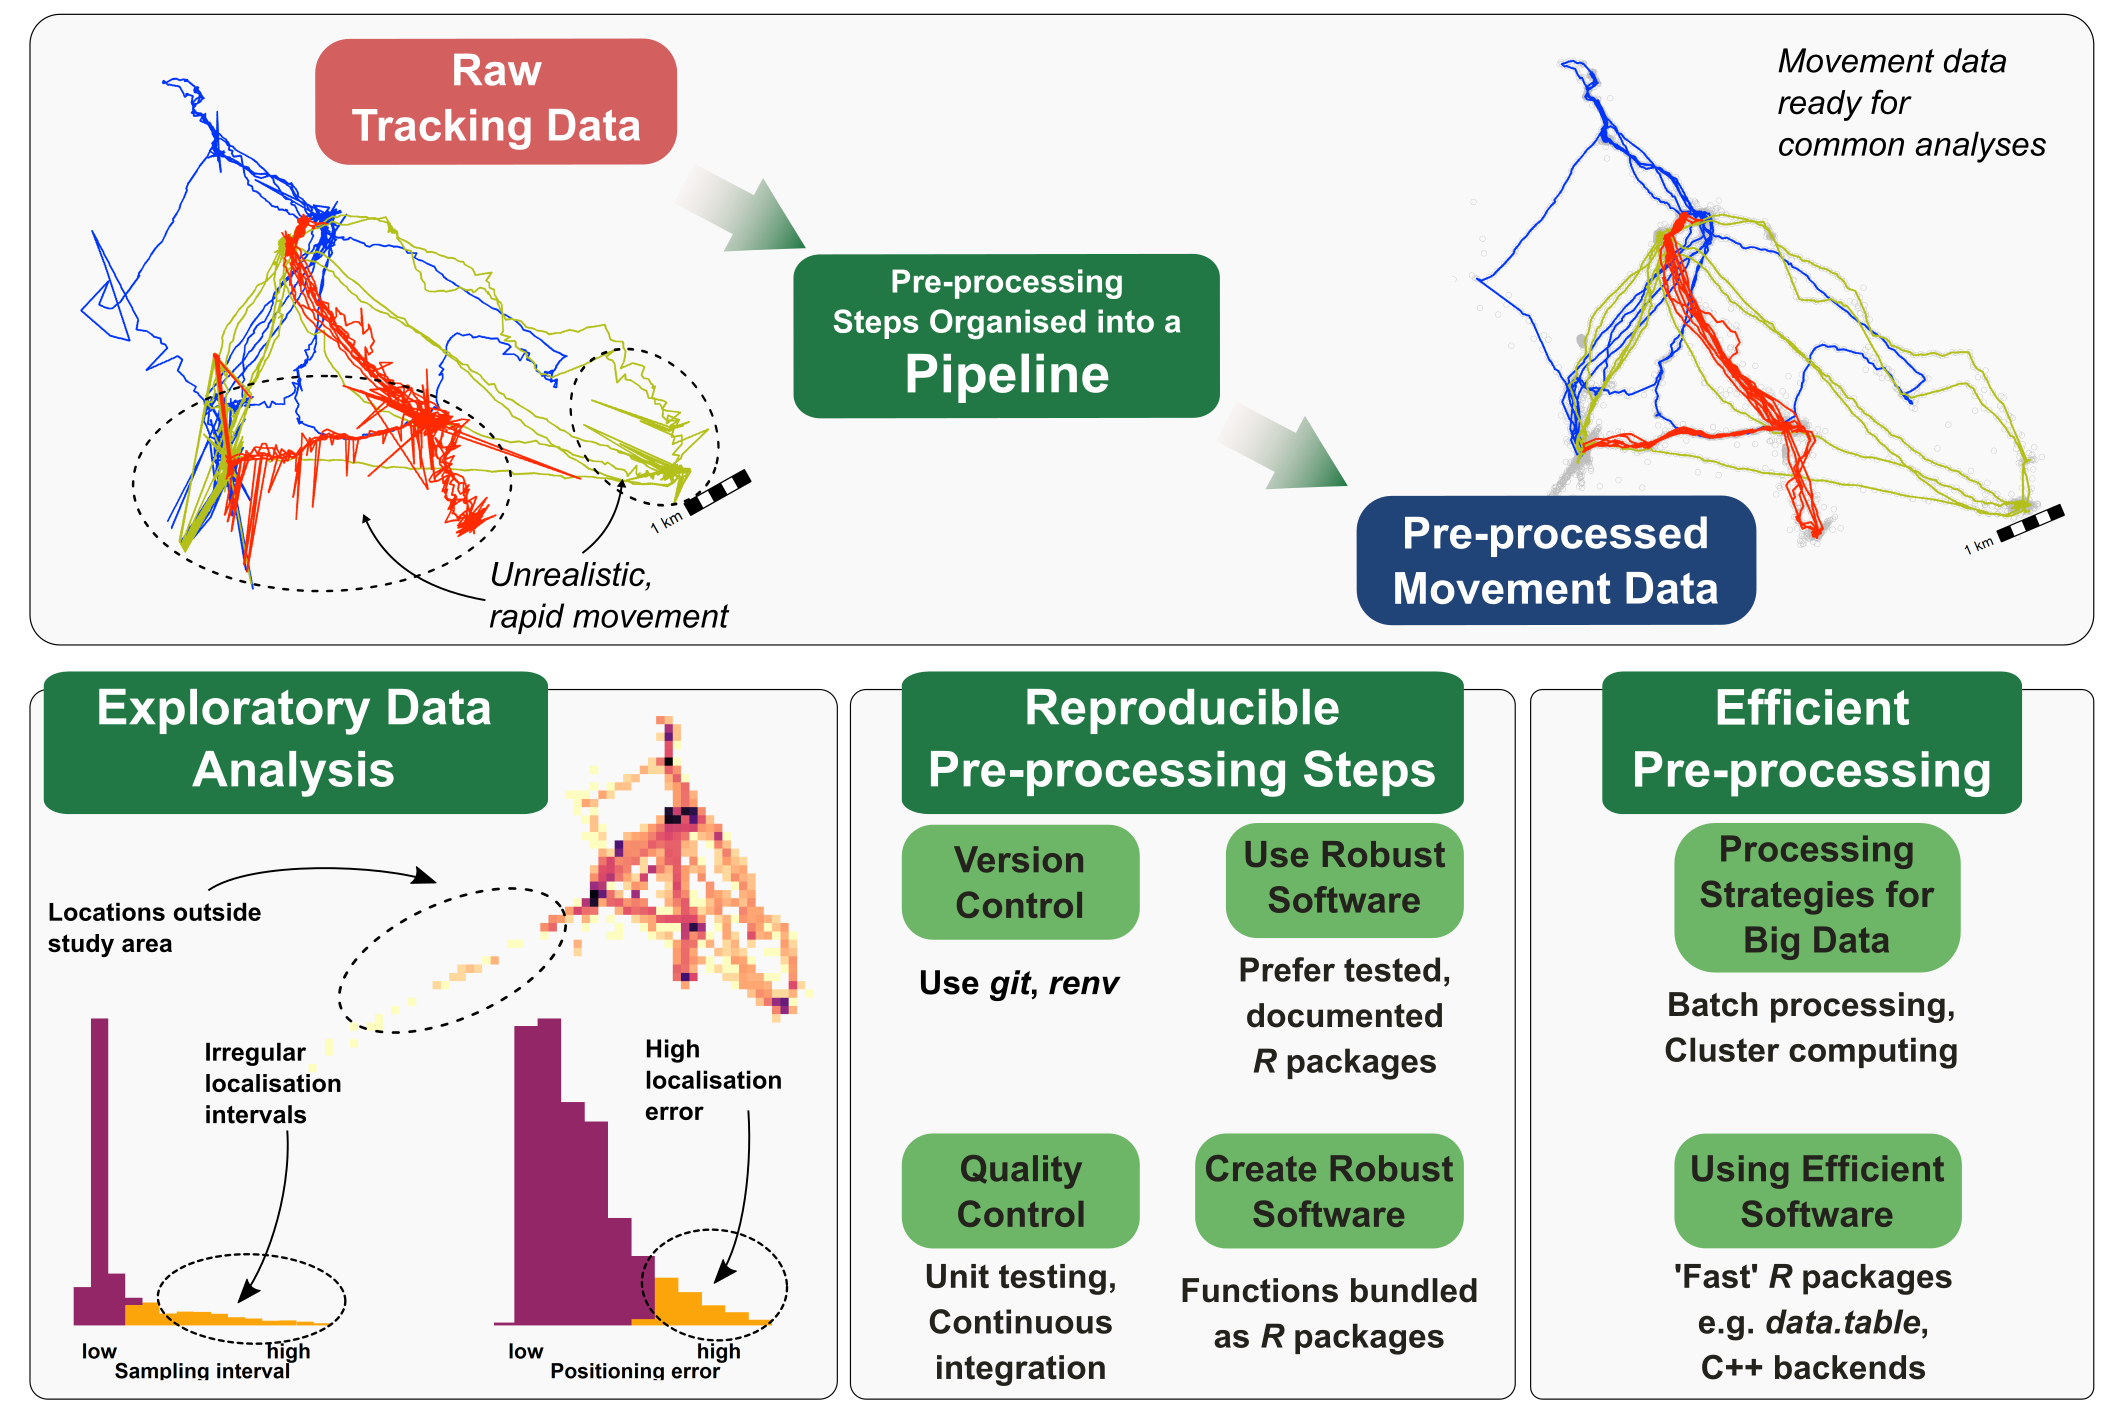
\includegraphics[width=13.5cm]{figures/preprocessing/fig_01.png}
        \end{addmargin}
        \caption{
            {\small
            \textbf{Some best-practices for pre-processing high-throughput tracking data.}
            Simple pre-processing of animal tracking data can improve the quality of animal tracking data, and the inferences that are drawn from it.
            % The organisation of pre-processing workflows into a `pipeline' --- a set of steps that users apply to prepare the data for a specific analysis --- can help make research more reproducible and reliable.
            Exploratory data analysis of representative subsets of the data can help to identify common issues with data quality, and to determine which pre-processing, steps such as filters and smooths, might be necessary (\textit{see also Fig.~\ref{fig2}}).
            Pre-processing steps implemented as programming code can be made reproducible and shareable by following best-practices for software development: (i) tracking changes to the steps, and the software used, using version control (e.g. \textit{git}, \textit{renv}), (ii) preferring pre-existing tools, such as \textit{R} packages, which are well documented and tested, (iii) encapsulating custom-written code as functions, and bundling related functions into a package, and (iv) checking the quality of both custom-written code (e.g. by testing functions), and the overall pipeline (e.g. data visualisation).
            The efficiency of pre-processing steps can be increased by using strategies for dealing with large datasets, such as batch processing, or using a computing cluster.
            The use of existing tools optimised for large datasets, or by writing code in a `fast' language such as \textit{C++}, can also speed up the pre-processing of large datasets (see main text for examples).
            % See the \textit{Worked Out Example} on Egyptian fruit bats, as well as Supplementary Material 1, for more details on implementing pipelines.
            % Fig.~\ref{fig2} shows an example of such a pipeline.
        }
        }
        % \end{addmargin}
        \label{fig1}
        % \end{addmargin}
    \end{figure}

    Exploratory data analysis should be the first step towards pre-processing movement data \citep[see Fig.~\ref{fig1};][]{slingsby2016}.
    Researchers with very large datasets of perhaps millions of rows should ideally select a representative subset of these data for exploratory data analysis, including individuals of different species, sexes, or seasonal cohorts.
    Examples of exploratory data analysis include plotting heatmaps of the number of observations per unit area across the study site (Fig.~\ref{fig1}).
    Histograms of the location error estimates, plotting the linear approximations of animal paths between observations, and histograms of the sampling interval can help determine how data need to be treated so as to minimise location errors and improve computational tractability (Fig.~\ref{fig1}).
    While pre-processing steps required for datasets will differ between studies and tracking technologies, we elaborate upon candidate steps and their parameterisation in following sections (see also Fig.~\ref{fig2}).

    Following exploratory data analysis and the parameterisation of data cleaning steps, the specific implementation of these steps should be made reliable and reproducible.
    Since reproducing pre-processing steps can be challenging when using only written descriptions from published articles, providing the code to implement pre-processing steps reduces ambiguity and increases reproducibility \citep{haddaway2015}.
    For technically advanced users, the best-practices here are \textit{(i)} to implement pre-processing steps as `functions', \textit{(ii)} to collect related functions --- e.g. for similar kinds of data --- into a software `package', \textit{(iii)} to `test' that the functions handle input as expected, and \textit{(iv)} implement `version control' throughout, such that the process of development is documented \citep[Fig.~\ref{fig1};][]{wickham2015,alston2020,perez-riverol2016}.

    As an example, our \textit{atlastools} package incorporates these best-practices, and may be used as a reference \citep[][]{gupte2020a}.
    We have written each pre-processing step as a separate function, and each of these functions is tested, usually on simulated data, but in some cases also on empirical data \citep[][see the directory \textit{tests/} in the associated Zenodo repository]{wickham2015}.
    Finally, logging error messages is crucial when passing data through a pipeline, helping determine which data subsets could not be handled as expected, and why.
    Users who would prefer to rely on pre-existing toolsets and methods can use \textit{R} packages that follow these best-practices, such as \textit{move} \citep{kranstauber2011}, and \textit{sftrack} \citep{boone2020}.

    The large size of modern, high-throughput animal tracking data means that the computational challenge can often be \textit{the} main challenge in working with these data.
    For beginning users, organising their workflows so that they process subsets of the data (such as one individual) at a time can help overcome limitations on working memory.
    Animal tracking data stored in a relational database \citep[e.g. SQL databases][]{codd1970}, for example, can be broken into meaningful subsets based on individual identity and tracking season.
    These smaller subsets can then be loaded into working memory, pre-processed, and saved in a separate location (see Supplementary Material 1, Section 2 for a worked out example on an SQL database).
    Using existing tools optimised for tabular data, such as the \textit{R} package \textit{data.table} \citep{dowle2020}, can also speed up computation; \textit{atlastools} is built using \textit{data.table} for this reason.

    More advanced users seeking substantial speed gains might wish to look into parallel-processing, and process each subset of the data independently of the full dataset, for example by using a computing cluster \citep[see also][for an alternative]{zjdai2021}.
    Finally, another advanced method, used by popular packages such as \textit{move} \citep{kranstauber2011} and \textit{recurse} \citep{bracis2018}, is to write one's own methods in a `fast' low-level language, such as \textit{C++}, and link these to \textit{R} \citep[][]{eddelbuettel2013}; see also \textit{adehabitatLT}, which is written partially in \textit{C} \citep{calenge2006}.
    Beginning practitioners can organise their workflows around these packages to benefit from the features they incorporate.

    \section*{Pre-processing Steps, Usage, and Simulating Data}

    \subsection*{An Overview of Pre-processing Steps and \textit{atlastools}}

    In the sections that follow, we lay out pre-processing techniques for raw high-throughput tracking data, and demonstrate working examples of these techniques, which we have collected in the \textit{R} package \textit{atlastools} (see Fig.~\ref{fig2}).
    Our package is aimed at getting `raw data' to the `analysis' stage identified by Joo et al. (2020) in their review of \textit{R} packages in movement ecology.
    The package is based on \textit{data.table}, a fast implementation of data frames; thus it is compatible with a number of data structures from popular packages including \textit{move}, \textit{sftrack}, and \textit{ltraj} objects, which can be converted to data frames \citep[][]{kranstauber2011,boone2020,calenge2009}.
    Our package functions are suitable for use with both regularly sampled data, as well as data with missing observations.

    We cover, first, the use of simple \textit{\textbf{Spatio-Temporal Filters}} to select positions within a certain time or area.
    Next, we show how users can \textit{\textbf{Reduce Location Errors}} by removing unreliable positions based on a system-specific error measure, or by the plausibility of associated movement metrics, such as speed and turning-angle \citep{seidel2018, calenge2009}.
    We then show how users can tackle small-scale location errors by applying a \textit{\textbf{Median Smooth}}, and users who need uniformly sampled data, can undertake \textit{\textbf{Data Thinning}} by either aggregation or subsampling.
    At this stage, the data are ready for a number of popular statistical treatments such as Hidden Markov Model-based classification \citep{michelot2016,langrock2012}.
    Finally, we show how users wishing simple, efficient segmentation-clustering of points where the animal showed prolonged residence, can classify their data into `residence patches' \citep{barraquand2008, bijleveld2016} based on the movement ecology of their study species, after filtering out travelling segments (see \textit{\textbf{System-Specific Pre-Processing Tools}}).

    These pre-processing techniques and package were designed with ATLAS systems in mind, motivated to meet the rapid growth of studies using this high-throughput system worldwide: in Israel \citep{toledo2014, toledo2016, toledo2020, corl2020, vilk2021}, the UK \citep{beardsworth2021a, beardsworth2021b}, and the Netherlands \citep[][Bijleveld et al. \textit{in prep.}]{beardsworth2021}. 
    However, the principles and functions presented here are ready for use with other massive high-resolution data collected by GPS \citep[e.g.][]{papageorgiou2019}, reverse-GPS \citep[e.g.][]{aspillaga2021} or any other high-throughput tracking system .
    Users may construct a pre-processing pipeline comprising of all the techniques we cover, or implement the modules most suitable for their data.
    Users are advised to visualise their data throughout their workflow, and especially to perform thorough exploratory data analysis, to check for evident location errors or other issues \citep{slingsby2016}.

    \begin{figure}
        \centering
        \begin{addmargin}{-.3\textwidth}%[-.3\textwidth]
        \centering
        \captionsetup{width=13.5cm}
        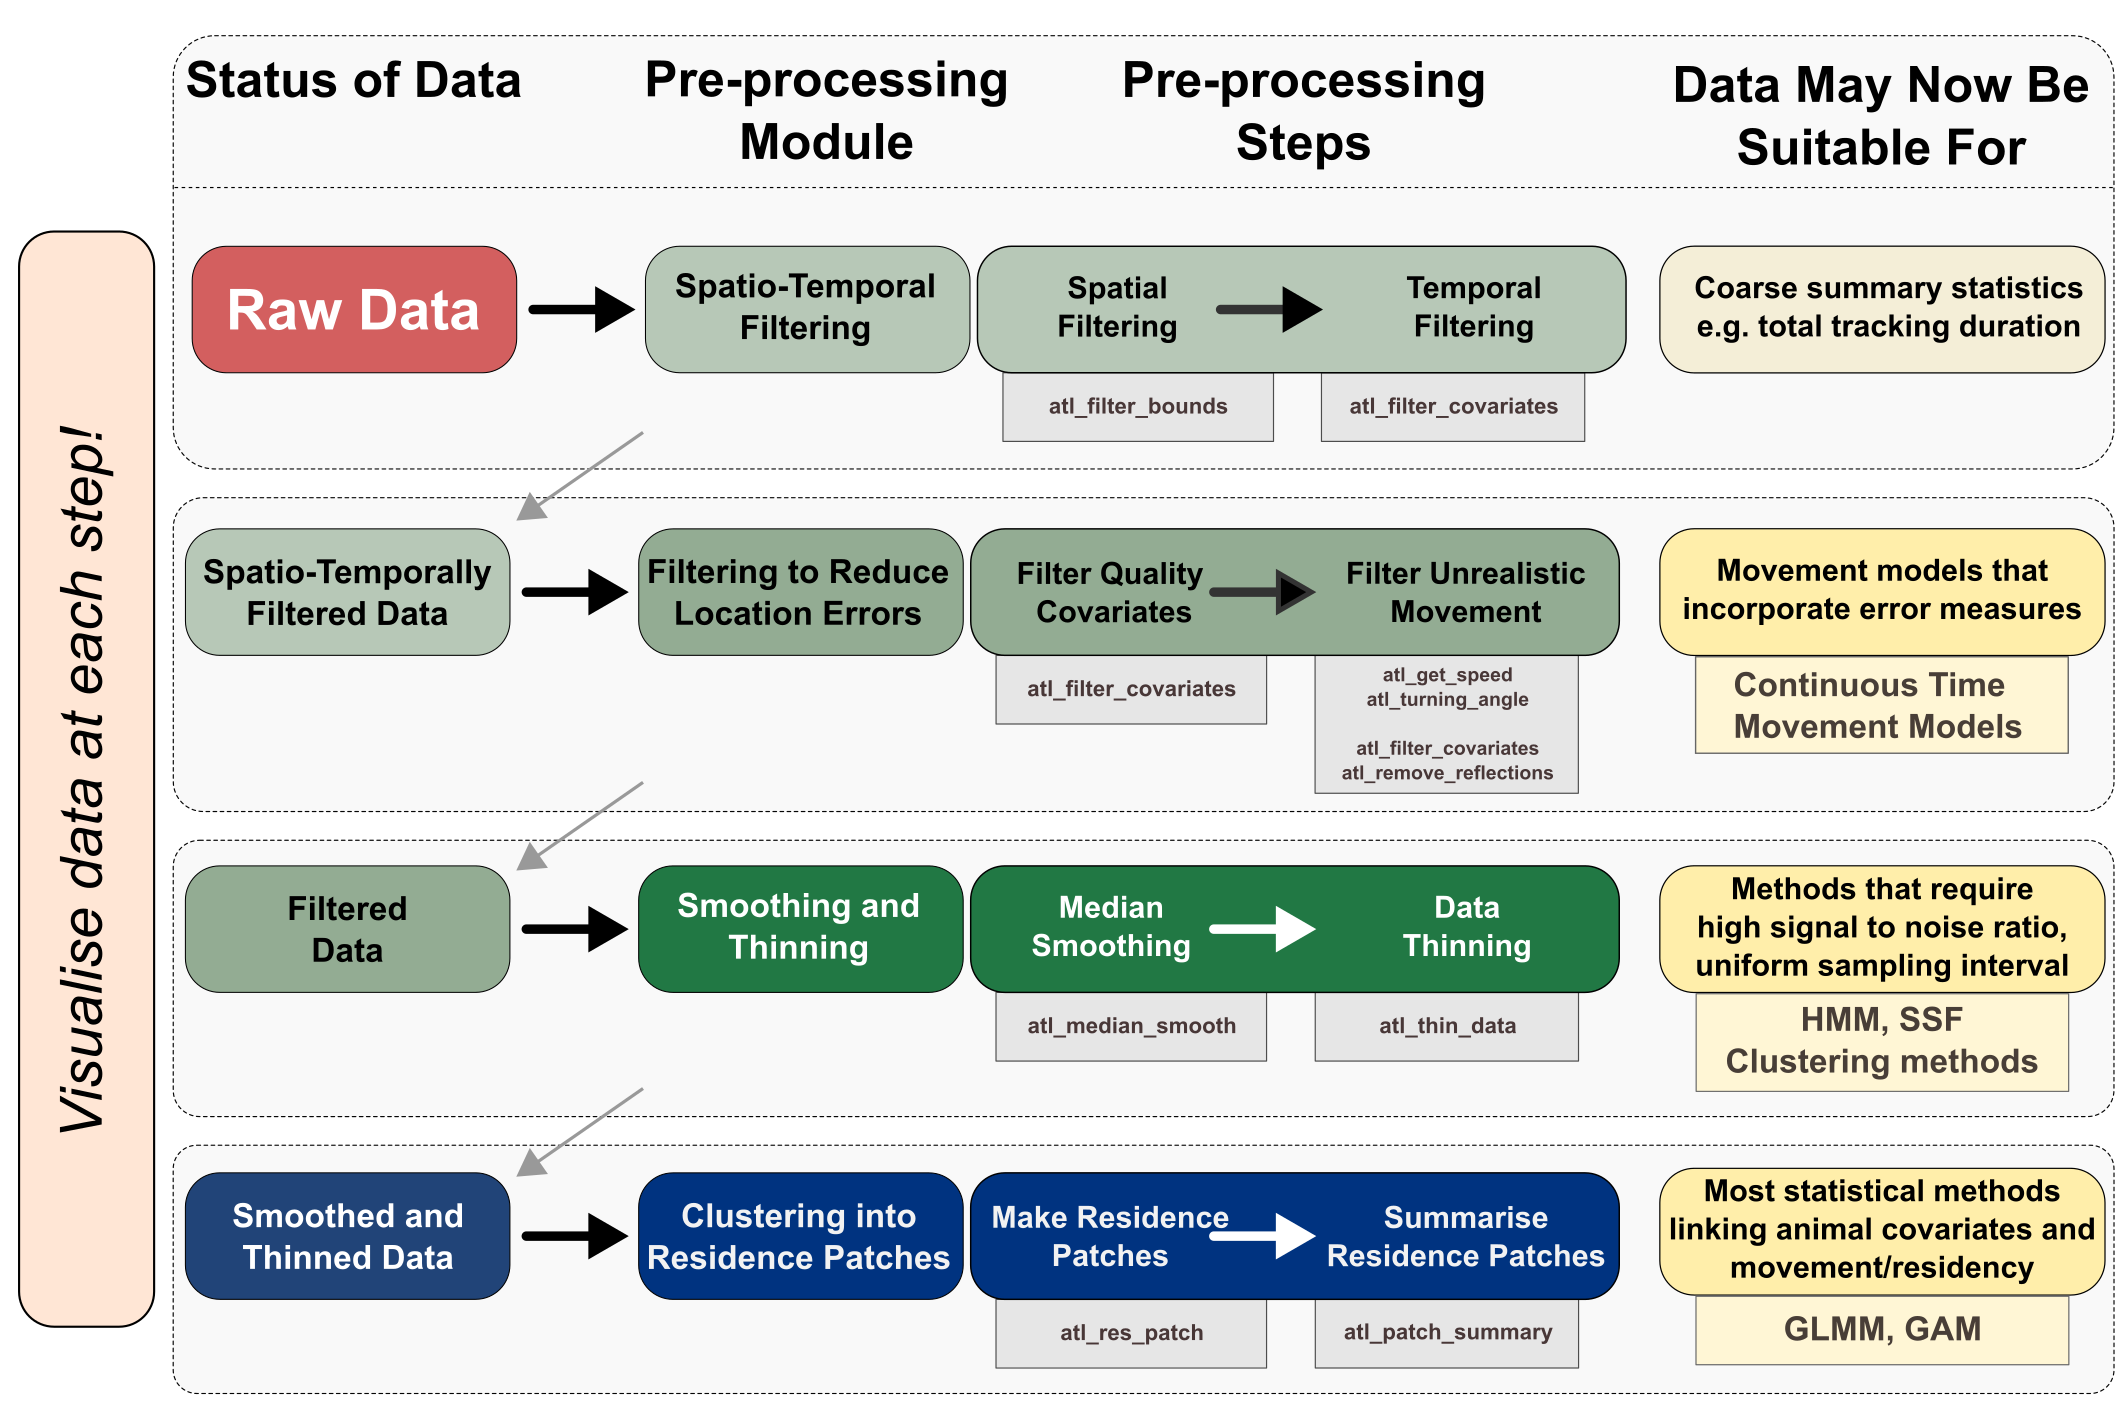
\includegraphics[width=13.5cm]{figures/preprocessing/fig_02.png}
        \end{addmargin}
        \caption{
            \textbf{An example of a modular pipeline for pre-processing high-throughput tracking data from raw localisations to cleaned data, and optionally into residence patches.}
            Users should apply the appropriate pre-processing modules and the steps therein until the data are suitable for their intended analysis, some of which are suggested here.
            The \textit{atlastools} function that may be used to implement each pre-processing step is shown in the grey boxes underneath each step.
            Popular statistical methods are shown underneath possible analyses (yellow boxes).
            Users are strongly encouraged to visualise their data and scan it for location errors as they work through the pipeline, always asking the question, could the animal plausibly move this way?
        }
        \label{fig2}
    \end{figure}

    \subsection*{Simulating Data to Demonstrate Pre-Processing Steps}

    To demonstrate pre-processing steps, we simulated a realistic movement track of 5,000 positions using an unbiased correlated velocity model (UCVM) implemented via the \textit{R} package \textit{smoove} \citep[][see Fig. 3.a]{gurarie2017}.
    We added four kinds of error to the simulated track: (i) normally distributed small-scale offsets to the X and Y coordinates (small-scale error), (ii) normally distributed large-scale offsets to a random subset (0.5 \%) of the positions (spikes), (iii) large-scale displacement of a continuous sequence of 300 of the 5,000 positions (prolonged spikes; indices 500 -- 800), and (iv) we removed 10\% of the canonical track to simulate missing data (see Fig. 3.a).
    To demonstrate the residence patch method, we obtained data, in the form of 1,000 positions, from a mechanistic, individual-based simulation model, in which agents move using simple decision making rules, and can find high-productivity patches using only ephemeral cues, such as the density of prey-items and other competitors \citep{gupte2021a, netz2021}.
    The emergent, complex track structure is analogous to the foraging movements of animals, and provides a suitable challenge for the residence patch method and helps to demonstrate its generality.

    \section*{Spatio-Temporal Filtering}

    \subsection*{Spatial Filtering Using Bounding Boxes and Polygons}

    First, users should exclude positions outside the spatial bounds of a study area by comparing position coordinates with the range of acceptable coordinates (the bounding box), and removing positions outside them (Fig. 3.a; {\color{red} Listing} 1). 
    A bounding box filter does not require a geospatial representation such as a shapefile, and can help remove unreliable data from a tracking system that is less accurate beyond a certain range \citep[][]{beardsworth2021}.
    In some special cases, users may wish to remove positions \textit{inside} a bounding box, either because movement behaviour within an area is not the focus of a study, or because positions recorded within an area are known to be erroneous.
    An example of the former is studies of transit behaviour between features which can be approximated by their bounding boxes. 
    Instances of the latter are likely to be system specific, but are known from ATLAS systems. 
    Bounding boxes are typically rectangular, and users seeking to filter for other geometries, such as a circular or irregularly-shaped study area, need a geometric intersection between their data and a spatial representation of the area of interest (e.g. shapefile, geopackage, or \textit{sf}-object in \textit{R}).
    The \textit{atlastools} function \textit{atl\_filter\_bounds} implements both bounding box and explicit spatial filters, and accepts X and Y coordinate ranges, an \textit{sf}-polygon or multi-polygon object \citep{pebesma2018}, or any combination of the three to filter the data ({\color{red} Listing} 1).
    When both coordinate ranges and a polygon are provided, the data is first filtered by the ranges and then the polygon.
    The boolean function argument \textit{remove\_inside} determines whether positions inside the bounds are retained (\textit{FALSE}) or removed (\textit{TRUE}).

    % \begin{lst{\color{red} Listing}}[float,floatplacement=h!,language=R, style=customR, caption = {
    %     The \textit{atl\_filter\_bounds} function filters on an area defined by coordinate ranges, a polygon, or all three; it can remove positions outside (\textit{remove\_inside = FALSE}), or within the area (\textit{remove\_inside = TRUE}).
    %     The arguments \textit{x} and \textit{y} determine the X and Y coordinate columns, \textit{x\_range} and \textit{y\_range} are the filter bounds in a coordinate reference system in metres, and the data can be filtered by an \textit{sf-(MULTI)POLYGON}, which can be passed using the \textit{sf\_polygon} argument. 
    %     The output is a \textit{data.table}, which must be saved as an object (here, \textit{filtered\_data}).}]
    % filtered_data <- atl_filter_bounds(
    %                         data = data,
    %                         x = "X", y = "Y",
    %                         x_range = c(x_min, x_max),
    %                         y_range = c(y_min, y_max),
    %                         sf_polygon = your_polygon,
    %                         remove_inside = FALSE
    %                     )
    % \end{lst{\color{red} Listing}}

    \begin{figure}[h!]
        \centering
        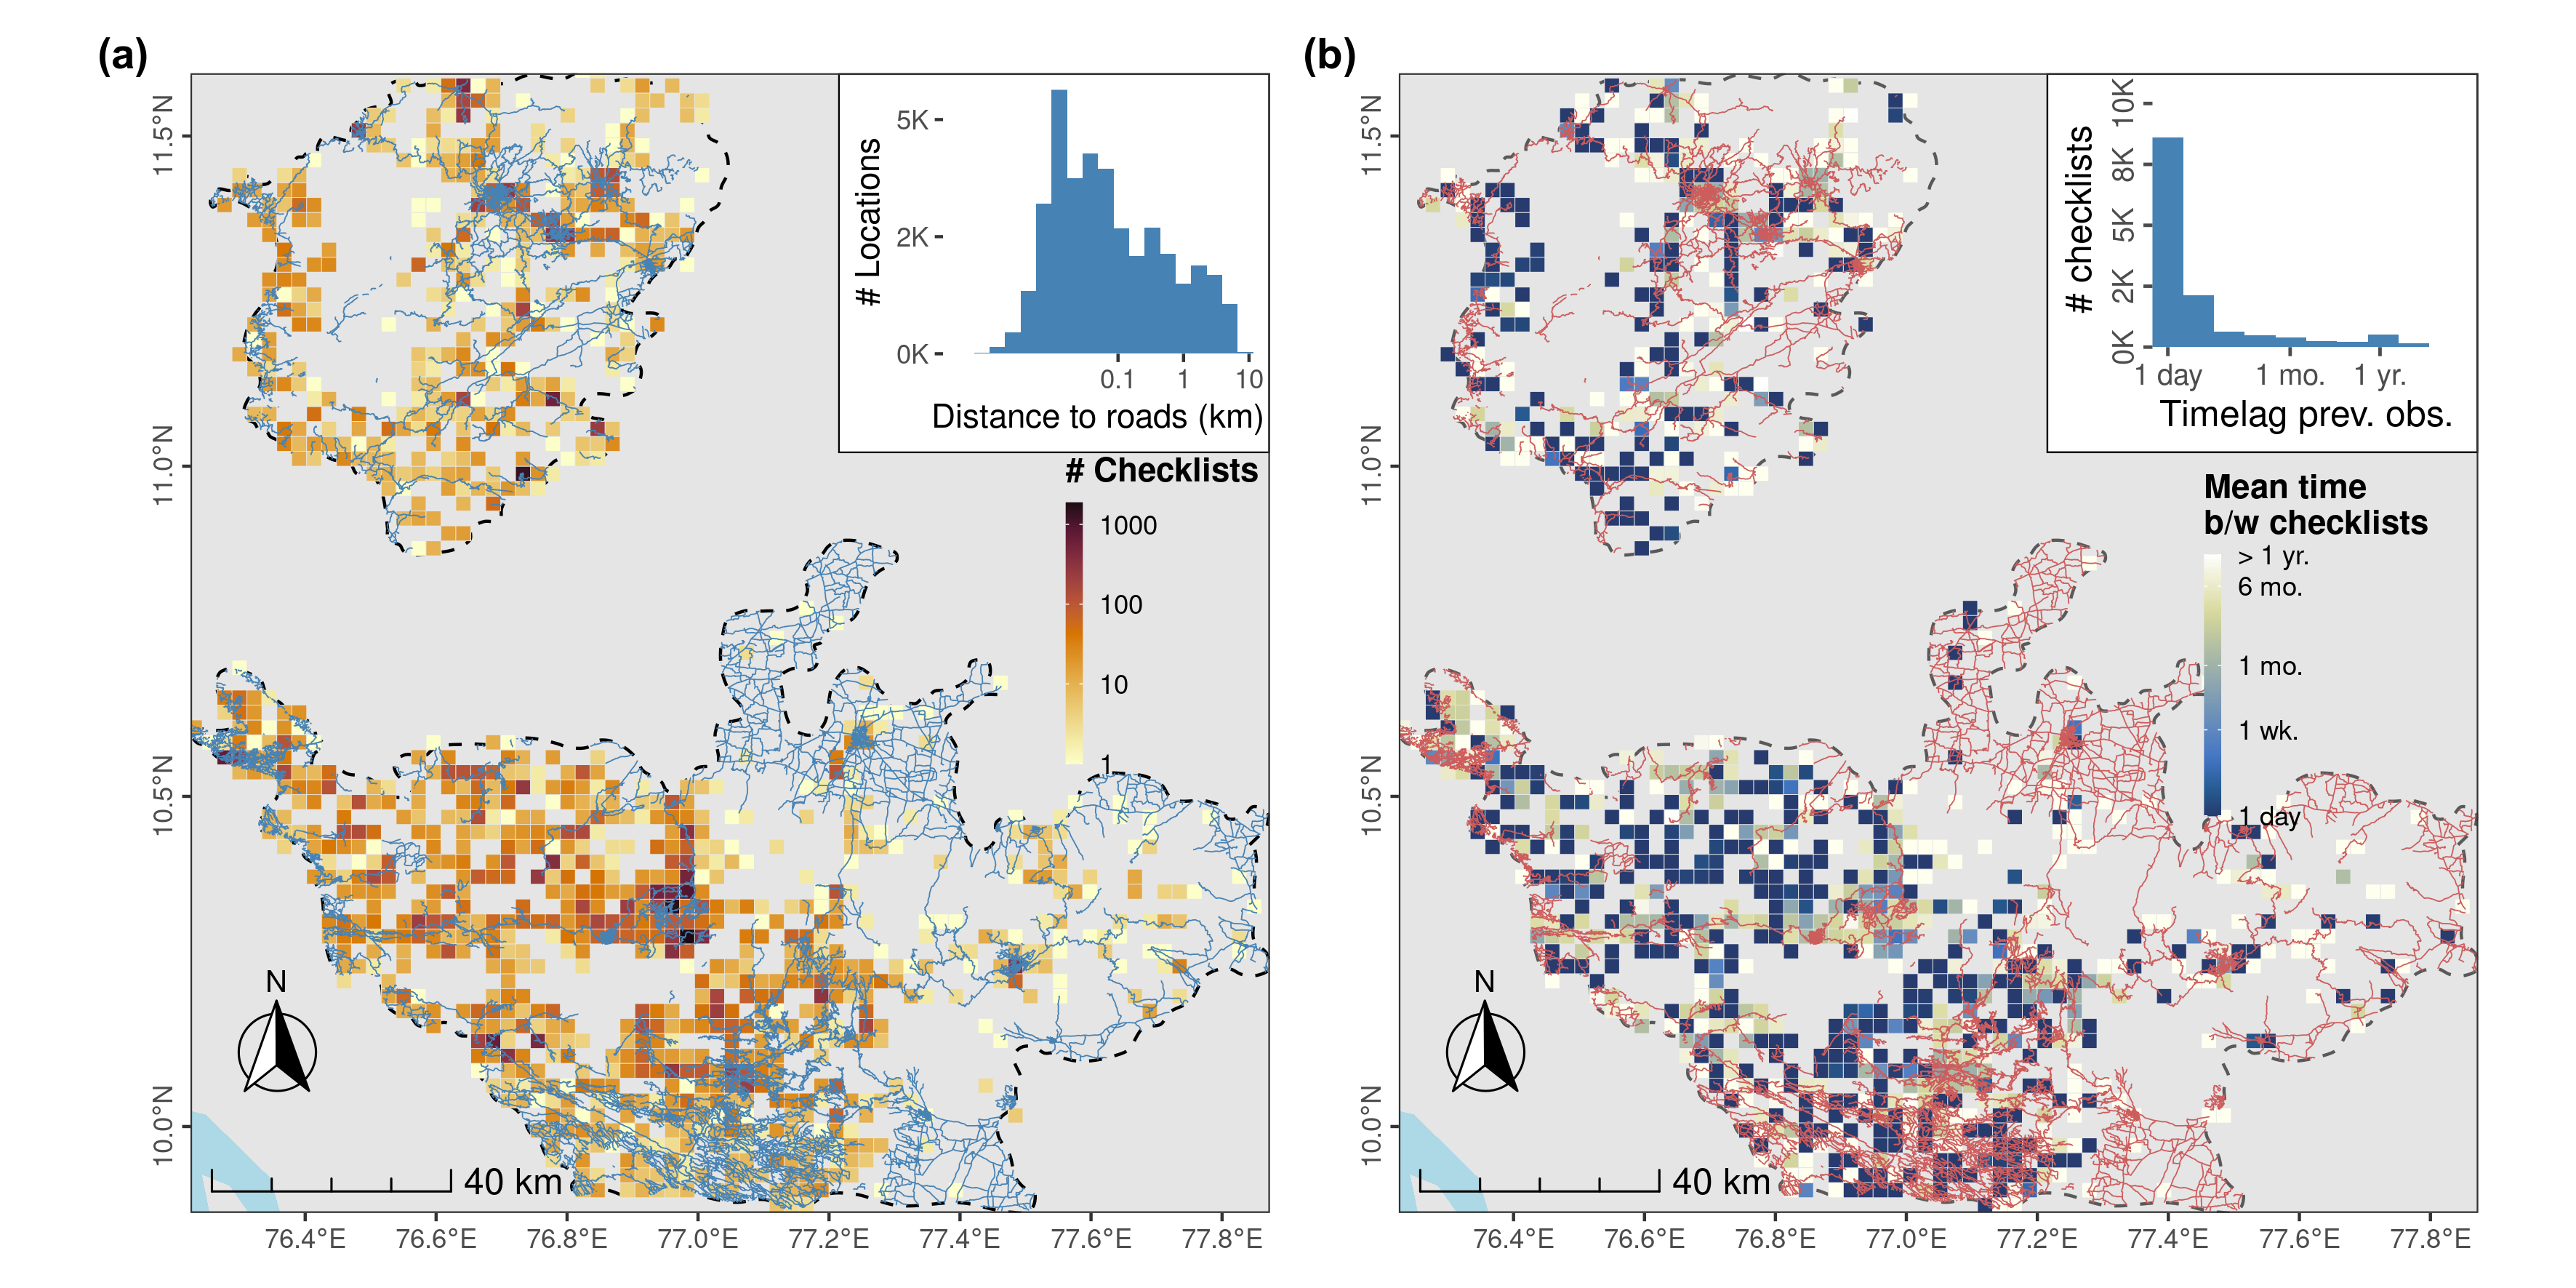
\includegraphics[width=0.9\textwidth]{figures/fig_03.png}
        \caption{
            \textbf{Simulated movement data showing four kinds of artificially added errors}.\\
            (i) Normally distributed small-scale error on each position, (ii) large-scale error added to 0.5\% of positions, (iii) 10\% of positions removed to simulate missing data, and (iv) 300 consecutive positions displaced to simulate a gross distortion affecting a continuous subset of the track.
            \textbf{(a)} Tracks can be quickly filtered by spatial bounds (dashed grey lines) to exclude broad regions (green = retained; grey = removed).
            \textbf{(b)} location error may affect single observations resulting in point outliers or `spikes' (red crosses and track segments), or continuous subsets of a track, called a `prolonged spike' (purple circles, top right), and both represent unrealistic movement.
            \textbf{(c)} Histograms of speed for the track (grey = small-scale errors, red = spikes), and the prolonged spike (purple) show that while spikes could be removed by filtering out positions with both high incoming and outgoing speeds and turning angles, prolonged spikes cannot be removed in this way, and should be resolved by conceptualising algorithms that find the bounds of the distortion instead.
            Users should frequently check the outputs of such algorithms to avoid rejecting valid data.
        }
        \label{fig:figure_filtering_data}
    \end{figure}

    \subsection*{Temporal and Spatio-temporal Filters}

    Tracking data might fail to properly represent an animal’s movement at certain times, for instance, data recorded before release, or data from shortly after release when the animal is still influenced by the stress of capture and handling.
    Periods of poor tracking quality may result from system malfunctions and unusual disturbances, and users may wish to exclude these data as well.
    Temporal filtering can exclude positions from intervals when data are expected to be unreliable for ecological inference, either due to abnormal movement behaviour or system-specific issues.  
    Temporal filters can be combined with spatial filters to select specific time-location combinations. 
    For example, studies of foraging behaviour of a nocturnal animal would typically exclude tracking data from the animal's daytime roosts (see \textit{Worked Out Example}).
    Users should apply filters in sequence rather than all at once, and visualise the output after each filtering step (`sanity checks'; see Supplementary Material Section 2).
    The atlastools function \textit{atl\_filter\_covariates} allows convenient filtering of a dataset by any number of logical statements, including querying data within a spatio-temporal range ({\color{red} Listing} 2).
    % This function can be used to easily filter timestamps in a range, as well as combine simple spatial and temporal filters.
    % It accepts a character vector of \textit{R} expressions that each return a logical vector (i.e., \textit{TRUE} or \textit{FALSE}; {\color{red} Listing} 2).
    The function keeps only those data which satisfy each of the filter conditions, and users must ensure that the filtering variables exist in their dataset in order to avoid errors.

    % \begin{lst{\color{red} Listing}}[float, language=R, style=customR, caption = {
    %     Data can be filtered by a temporal or a spatio-temporal range using \textit{atl\_filter\_covariates}. 
    %     Filter conditions are passed to the \textit{filters} argument as a character vector. 
    %     Only rows in the data satisfying \textit{all} the conditions are retained. 
    %     Here, the first example shows how nighttime data can be retained using a predicate that determines whether the value of `hour' is between 6 and 18, and also within a range of X coordinates.
    %     The second example retains ATLAS locations calculated using $>$ 3 base stations (\textit{NBS}), with location error (\textit{SD}) $<$ 100, and data between an arbitrary day 5 and day 8.
    %     }]
    % night_data <- atl_filter_covariates(
    %                     data = dataset,
    %                     filters = c(
    %                         "!inrange(hour, 6, 18)",
    %                         "between(x, x_min, x_max)"
    %                     )
    %                 )

    % filtered_data <- atl_filter_covariates(
    %                         data = data,
    %                         filters = c(
    %                             "NBS > 3",
    %                             "SD < 100",
    %                             "between(day, 5, 8)"
    %                         )
    %                     )                            
    % \end{lst{\color{red} Listing}}

    \section*{Filtering to Reduce Location Errors}

    \subsection*{Filtering on Data Quality Attributes}

    Tracking data attributes can be good indicators of the reliability of positions calculated by a tracking system \citep{beardsworth2021}.
    GPS systems provide direct measures of location error during localisation \citep[Horizontal Dilution of Precision, HDOP in GPS]{ranacher2016}, while  in reverse-GPS systems, a measure referred to as Standard Deviation (SD in many datasets), can be calculated from the variance-covariance matrix of each position as: $\text{SD} = \sqrt{\text{Var X} + \text{Var Y} + \text{Cov XY}}$ \citep[see details in][]{maccurdy2009, maccurdy2019, weiser2016, ranacher2016}.
    Tracking data can also include indirect indicators of data quality.
    For instance, GPS systems' location error may be indicated indirectly by the number of satellites involved in the localisation.
    In reverse-GPS systems too, the number of base stations involved in each localisation is an indirect indicator of data quality, and positions localised using more receivers are usually more reliable \citep[the minimum required for an ATLAS localisation is 3; see][]{weiser2016, beardsworth2021}.
    % A location error measure associated with each coordinate pair (similar to GPS HDOP) can be calculated and assigned to a new column \textit{SD} using the formula for the sum of correlated random variables
    % \begin{linenomath*}
    %     \begin{equation*}
    %         SD = \sqrt{{VARX} + {VARY} + 2 \times {COVXY}}
    %      \end{equation*}
    % \end{linenomath*}
    Unreliable positions can be removed by filtering on direct or indirect measures of quality using \textit{atl\_filter\_covariates} ({\color{red} Listing} 2).
    While filtering on direct quality attributes and unrealistic movement speeds (see below) will often be sufficient, filtering on indirect quality indicators is a strategy to consider when direct error measures are not available.

    \subsection*{Filtering Unrealistic Movement}

    Filtering on system-generated attributes may not remove all erroneous positions, and the remaining data may still include biologically implausible movement.
    Users are encouraged to visualise their tracks before and after filtering point locations, and especially to `join the dots' and connect consecutive positions with lines (Fig. 3.b).
    Whether the resulting track looks realistic is ultimately a subjective human judgement, but any decision to filter-out data must remain independent of the hypothesised movement behavior.
    This basic principle does not preclude explicitly integrating prior knowledge of the movement ecology of the study species to ask, `Does the animal move this way?'.
    Segments which appear to represent unrealistic animal movement are often obvious to researchers with extensive experience of the study system \citep[the non-movement approach; see][]{bjorneraas2010}.
    Since it is both difficult and prohibitively time consuming to exactly reproduce expert judgement when dealing with large volumes of tracking data from multiple individuals, some automation is necessary.
    Users should first manually examine a representative subset of tracks and attempt to visually identify problems --- either with individual positions, or with subsets of the track --- that persist after filtering on system-generated attributes.
    Once such problems are identified, users can conceptualise algorithms that can be applied to their data to resolve them.

    A common example of a problem with individual positions is that of point outliers or `spikes' \citep{bjorneraas2010}, where a single position is displaced far from the track (see Fig. 3.b).
    Point outliers are characterised by artificially high speeds between the outlier and the positions before and after \citep[called incoming and outgoing speed, respectively;][]{bjorneraas2010}, lending a `spiky' appearance to the track.
    Removing spikes is simple: remove positions with extreme incoming and outgoing speeds.
    Users must first define plausible upper limits of the study species' speed \citep{calenge2009, seidel2018}.
    Here, it is important to remember that speed estimates are scale-dependent; high-throughput tracking typically overestimates the speed between positions where the animal is stationary or moving slowly, due to small-scale location errors \citep{ranacher2016, noonan2019}. 
    Even after data with large location errors have been removed, it is advisable to begin with a liberal (high) speed threshold that excludes only the most unlikely speeds.
    Estimates of maximum speed may not always be readily obtained for all species, and an alternative is to use a data-driven threshold such as the 90\textsuperscript{th} percentile of speeds from the track.
    Once a speed threshold $S$ has been chosen, positions with incoming \textit{and} outgoing speeds $> S$ may be identified as spikes and removed.

    Some species can realistically achieve speeds $> S$ in fast transit segments when assisted by their environment, such as birds with tailwinds, and a simple filter on incoming and outgoing speeds would exclude this valid data.
    To avoid removing valid, fast transit segments while still excluding spikes, the speed filter can be combined with a filter on the turning angles of each position \citep[see][]{bjorneraas2010, calenge2009}.
    This combined filter assumes that positions in high-throughput tracking with both high speeds and large turning angles are likely to be due to location errors, since most species are unable to turn sharply at very high speed.
    Users can then remove those positions whose incoming and outgoing speeds are both $> S$, and where $\theta > A$ (sharp, high-speed turns), where $\theta$ is the turning angle, and $A$ is the turning angle threshold.
    Many other track metrics may be used to identify implausible movement and to filter data \citep{seidel2018}.
    At this early stage in pre-processing, track metrics should be considered provisional --- it is not until after smoothing and potentially resampling to a regular interval (see below), that calculated track metrics should be used for ecological inference.
    We show an implementation of spike removal using the \textit{atl\_filter\_covariates} function ({\color{red} Listing} 3).

    % \begin{lst{\color{red} Listing}}[float, language=R, style=customR, caption = {
    %     Filtering a movement track on incoming and outgoing speeds, and on turning angle to remove unrealistic movement.
    %     The functions \textit{atl\_get\_speed} and \textit{atl\_turning\_angle} are used to get the speeds and turning angles before filtering, and assigned to a column in the data (assignment of \textit{speed\_out} is not shown).
    %     The filter step only retains positions with speeds below the speed threshold $S$ \textit{or} angles above the turning angle threshold $\theta$, i.e., positions where the animal is slow but makes sharp turns, and data where the animal moves quickly in a relatively straight line.}]
    % data$speed_in <- atl_get_speed(
    %                     data,
    %                     x = "x", y = "y",
    %                     time = "time", 
    %                     type = c("in")
    %                 )

    % data$angle <- atl_turning_angle(
    %                     data,
    %                     x = "x", y = "y", 
    %                     time = "time"
    %                 )

    % filtered_data <- atl_filter_covariates(
    %                     data = data,
    %                     filters = c(
    %                         "(speed_in < S & speed_out < S) | angle < A"
    %                     )
    %                 )
    % \end{lst{\color{red} Listing}}

    Sometimes, entire subsets of the track may be affected by the same large-scale location error.
    For instance, multiple consecutive positions may be roughly translated (geometrically) away from the real track and form `prolonged spikes', or `reflections' (see Fig. 3.b).
    These cannot be corrected by targeted removal of individual positions, as in Bjørneraas et al.'s approach (2010), since there are no positions with both high incoming and outgoing speeds, as well as sharp turning angles, that characterise spikes.
    Since filtering individual positions will not suffice, algorithms to correct such errors must take a track-level view, and target the displaced sequence overall.
    Track-subset algorithms are likely to be system-specific, and may be challenging to conceptualise or implement.
    In the case of prolonged spikes, one relatively simple solution is identifying the bounds of displaced segments, and removing positions between them.
    This identification can be based on relatively simple rules --- for example, the beginning of a prolonged spike could be identified as a position with a high \textit{incoming} speed, but a low \textit{outgoing} speed, while the end of such a spike would have a low incoming, but a high outgoing speed.
    We have implemented an illustrative example of such an algorithm in the form of track-subset filtering for prolonged spikes using the \textit{atlastools} function \textit{atl\_remove\_reflections} (see the \textit{atlastools} documentation for details on the algorithm).
    Users are strongly encouraged to visualise their data before and after applying such algorithms; as these methods are not foolproof, and data that are heavily distorted by errors affecting entire track-subsets should be used with care when making further inferences.

    % % \begin{lst{\color{red} Listing}}[float, language=R, style=customR, caption = {
    % %     Removing unrealistic movement in the form of prolonged spikes from a movement track. 
    % %     The important function arguments here are \textit{point\_angle\_cutoff} ($A$), \textit{reflection\_speed\_cutoff} ($S$), and \textit{est\_ref\_len}, the maximum number of positions after the inner bound that are candidates for the end of the prolonged spike, i.e., the outer bound. 
    % %     If the prolonged spike ends after less than $N$ positions, the true end point is used as the outer bound of the spike.
    % %     However, the algorithm behind this function fails when the prolonged spike ends after more than $N$ positions. 
    % %     Users are advised to use a liberally large value of N in the \textit{est\_ref\_len} argument; 1,000 may be appropriate for 3s interval data.
    % %     Further, users are cautioned against relying on such algorithms for severely distorted data.}]
    % % filtered_data <- atl_remove_reflections(data = track_data,
    % %                        x = "x", y = "y", time = "time",
    % %                        point_angle_cutoff = A,
    % %                        reflection_speed_cutoff = S,
    % %                        est_ref_len = N)
    % % \end{lst{\color{red} Listing}}

    \section*{Smoothing and Thinning Data}

    \subsection*{Median Smoothing}

    After filtering out large location errors, the track may still look `spiky’ at small scales, and this is due to smaller location errors that are especially noticeable when the individual is stationary or moving slowly \citep{noonan2019}.
    These smaller errors are challenging to remove since their attributes (such as speed and turning angles) are within the expected range of movement behaviour for the study species. 
    The large data volumes of high-throughput tracking allow users to resolve this problem by smoothing the positions. 
    The most basic `smooths' work by approximating the value of an observation based on neighbouring values.
    For a one-dimensional series of observations, the neighbouring values are the $K$ observations centred on each index value $i$.
    The range ${i - (K-1)/2} \ldots {i + (K-1)/2}$ is referred to as the moving window as it shifts with $i$, and $K$ is the moving window size.
    A common smooth is nearest neighbour averaging, in which the value of an observation $x_i$ is the average of the moving window $K$.
    The median smooth is a variant of nearest neighbour averaging which uses the median rather than the mean, and is more robust to outliers (\citeauthor{tukey1977} 1977).
    The median smoothed value of the X coordinate, for instance, is
    %
    % \begin{linenomath*}
        % \begin{equation*}
        $$
            X_i = \text{Median}(X_{i - (K-1)/2} \ldots X_{i + (K-1)/2}).
        $$
            % \end{equation*}
    % \end{linenomath*}
    %
    Users can apply a median smooth with an appropriate $K$ independently to the X and Y coordinates of a movement track to smooth it (see Fig. 4.a -- e).
    The median smooth is robust to even very large temporal and spatial gaps, and does not interpolate between positions when data are missing. 
    Thus it is not necessary to split the data into segments separated by periods of missing observations when applying the filter (see Fig. 4).

    Some data sources, such as GPS, provide tracks that have already been smoothed in quite sophisticated ways, such as with a Kalman filter, making a median smooth unnecessary \citep{kaplan2005}.
    Furthermore, smoothing is not a panacea for data quality issues, and has its drawbacks.
    Smoothing does not change the number of observations, but does decouple the coordinates from some of their attributes.
    For instance, smoothing breaks the relationship between a coordinate and the location error estimate around it (VARX, VARY, and SD in ATLAS systems).
    Since the X and Y coordinates are smoothed independently, the smoothed coordinates of an observation will likely differ from all the coordinates used to compute the smoothed value.
    Any position covariates (e.g. environmental values such as landcover or elevation) obtained before smoothing should be replaced with the covariates obtained at the smoothed coordinates.
    Similarly, instantaneous track metrics, such as speed and turning angle, should also be updated at this stage to reflect the smoothed coordinates.
    Furthermore, the location error estimate around each coordinate, and around the localisation overall, become invalid and should be ignored.
    This makes subsequent filtering on measures of data quality unreliable, and smoothed data are unsuitable for use with methods that model location uncertainty \citep{noonan2019, fleming2014a, fleming2020, calabrese2016}.
    Thus, when applying location error modelling methods, users should ensure that the error measure bears a mechanistic relationship with the location estimate \citep[see][ for more details]{fleming2020, noonan2019}.
    Additionally, excessively large $K$ may result in a loss in detail of the individual's small-scale movement (compare Fig. 4.e with 4.a).
    Users must themselves judge how best to balance large-scale and small-scale accuracy, and choose $K$ accordingly.
    Median smoothing is provided by the \textit{atlastools} function \textit{atl\_median\_smooth}, with the only option being the moving window size, which must be an odd integer ({\color{red} Listing} 4).

    % \begin{lst{\color{red} Listing}}[float, language=R, style=customR, caption = {
    %     Median smoothing a movement track using the function \textit{atl\_median\_smooth} function with a moving window \textit{K = 5}. 
    %     Larger values of $K$ yield smoother tracks, but $K$ should always be some orders of magnitude lower than the number of observations.}]
    % atl_median_smooth(
    %     data = track_data,
    %     x = "x", y = "y",
    %     time = "time",
    %     moving_window = 5
    % )
    % \end{lst{\color{red} Listing}}

    \begin{figure}[h!]
        \centering
        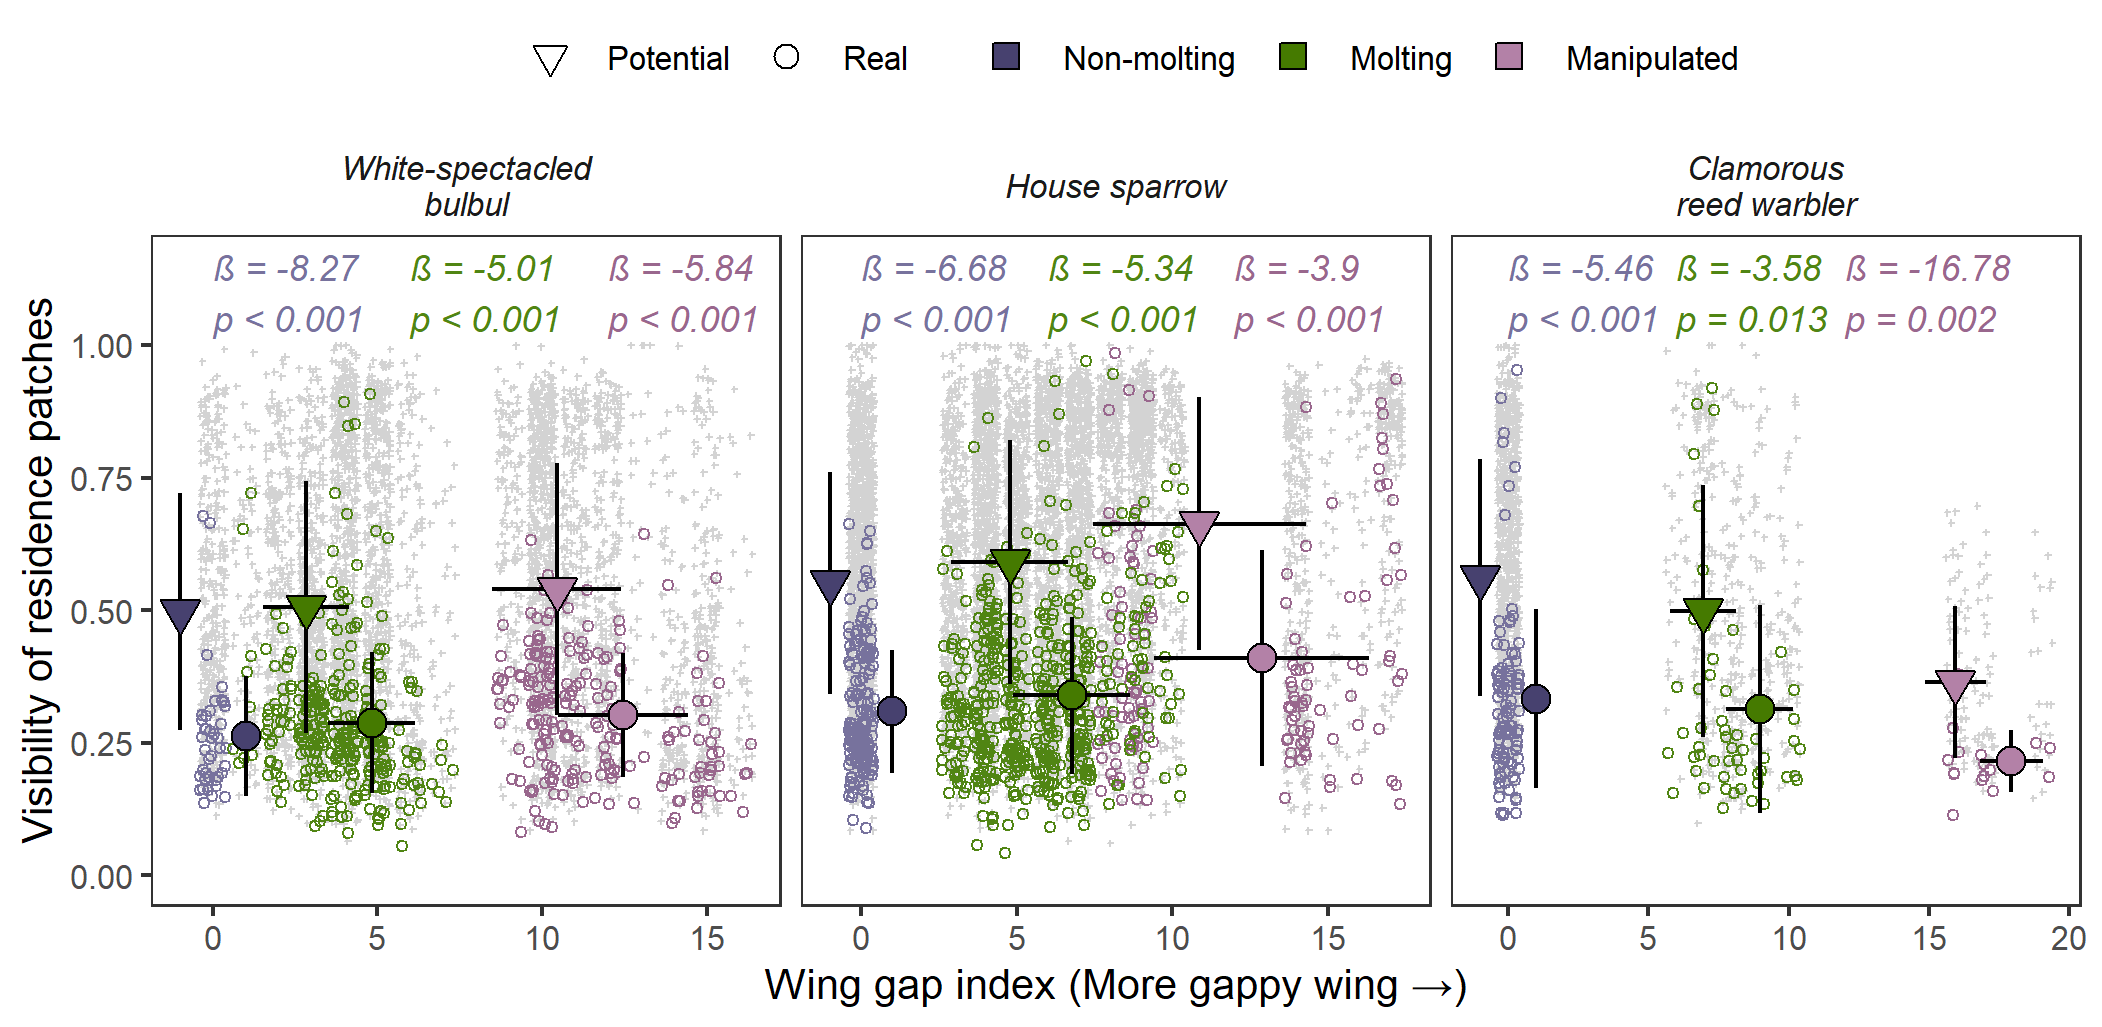
\includegraphics[width=0.95\textwidth]{figures/fig_04.png}
        \caption{
            \textbf{Median smoothing position coordinates reduces small-scale location error in tracking data.}\\
            The goal of this step is to approximate the simulated canonical track (black line, \textbf{(a)}), given positions with small-scale error that remains after filtering in previous steps (green points).
            \textbf{(b)} Median smoothing the position coordinates (green points, in \textbf{(a)}) over a moving window ($K$) of 21 positions gives a good approximation (blue line) of the canonical track, and is a significant improvement on the unsmoothed track (grey lines and points).
            While $K$ should usually be at least two orders of magnitude less than the number of positions in the track, users are cautioned that there is no correct $K$, and they must subjectively choose a $K$ which most usefully trades small-scale details of the track for large-scale accuracy.
            Here, smoothing with a $K$ of \textbf{(c)} 5 (dark grey line) and \textbf{(d)} 11 (blue line), leads to a jagged track, compared to the true path in (a), and the distance moved by the animal would be overestimated.
            \textbf{(e)} Using extremely large values of $K$ (101) may lead to a loss of both large and small scale detail (red line).
            Across panels, grey lines and points show the track without smoothing.
        }
        \label{fig:figure_median_smooth}
    \end{figure}

    \subsection*{Thinning Movement Tracks}

    Most data at this stage are technically ‘clean’, yet the volume alone may pose challenges for lower-specification or older hardware and software if these are not optimised for efficient computation.
    Thinning data i.e., reducing their volume, need not compromise researchers' ability to answer ecological questions; for instance, proximity-based social interactions lasting 1 -- 2 minutes would still be detected on thinning from a sampling interval of 1 second to 1 minute \citep[][]{aspillaga2021a}.
    Thinning data also does not imply that efforts to collect high-throughput movement data are ‘wasted’, as rich movement datasets enable more detailed and more accurate representation of the true track, as elaborated above. 
    Indeed, some analyses require that temporal auto-correlation in the data be broken by subsampling the data to a lower resolution; these include traditional kernel density estimators for animal home-range, as well as resource selection functions \citep{fleming2014a,manly2007,dupke2017}.
    Furthermore, a number of powerful methods in movement ecology, including Hidden Markov Models and integrated Step-Selection Analysis recommend uniform sampling intervals \citep{avgar2016,langrock2012,michelot2016}.
    Finally, subsampling data may be an important strategy in exploratory data analysis; for instance, it allows researchers to determine whether computationally intensive methods, such as distance and speed estimates from continuous time movement model fitting, are required for their data, or whether the movement metrics stabilise at a certain time scale \citep[][]{noonan2019}.
    Two plausible approaches here are subsampling and aggregation, and both approaches begin with identifying time-interval groups (e.g. of 1 minute).
    Subsampling picks one position from each time-interval group while aggregation involves computing the mean or median of all system-generated attributes for positions within a time-interval group.
    Here again, users should repeat the extraction of any environmental covariates for the thinned data, and may wish to obtain the mean values in a radius aroung the locations, rather than point estimates alone.
    Both approaches yield one position per time-interval group (Fig. 5.a).
    Categorical variables, such as the habitat type associated with each position, can be aggregated using a suitable measure such as the mode.
    We caution users that thinning causes an extensive loss of small-scale detail in the data, and should be used carefully.

    Both aggregation and subsampling have their relative advantages. 
    The aggregation method is less sensitive to selecting point outliers by chance than subsampling.
    However, to account for location error with methods such as state-space models \citep{jonsen2003, jonsen2005, johnson2008} or continuous time movement models \citep{fleming2014a, noonan2019, gurarie2017, calabrese2016, fleming2020}, correctly propagating the location error is important, and subsampling directly propagates these errors without further processing.
    In reverse-GPS systems systems the location error is calculated from the variance-covariance matrix of the coordinates of candidate positions considered by the location solver \citep{weiser2016}; this is equivalent to GPS systems' HDOP \citep{ranacher2016}.
    In the aggregation method, the location error around each coordinate provided by either GPS or reverse-GPS systems can be propagated --- assuming the errors are normally distributed --- to the averaged position as the sum of errors divided by the square of the number of observations contributing to each average ($N$):
    % \begin{linenomath*}
        $$
            \text{Var}(X)_{agg} = \left( \sum_{i=1}^{i=N} \text{Var}(X)_i \right) / N ^ 2
        $$
    % \end{linenomath*}
    Similarly, the overall location error estimate for the average of $N$ positions in a time-interval can be calculated by treating it as a variance. For instance, the ATLAS error and GPS error measures (SD and HDOP, respectively) can be aggregated as:
    % \begin{linenomath*}
        $$
            SD_{agg} \ or \ HDOP_{agg} = \sqrt{ \left( \sum_{i=1}^{i=N} SD_i^2 \ or \ HDOP_i^2 \right) / N ^ 2  }
        $$
    % \end{linenomath*}

    Users may question why thinning, which can obtain consensus positions over an interval and also reduce data-volumes should not be used directly on the raw data.
    %%
    We caution that thinning prior to excluding unrealistic movement and smoothing (Fig 5.b) can lead to preserving artefacts in the data, and estimates of essential metrics --- such as straight-line displacement (and hence, speed) --- that are substantially different from the true value \citep[see Fig. 5.c;][]{noonan2019}.
    In our example, the data with errors would have to be thinned to \sfrac{1}{30}\textsuperscript{th} of its volume for the median speed of the thinned data to be comparable with the overall median speed --- this is an undesirable step if the aim is fine-scale tracking.
    Additionally, the optimal level of thinning can be difficult to determine, especially if there is wide individual variation in movement behaviour, and the mis-estimation of track metrics from inappropriately thinned data could have consequences for the implementation of subsequent filters based on detecting unrealistic movement.
    However, thinning before data-cleaning has its place as a useful step before exploratory visualisation of the movement track, since reduced data-volumes are easier to handle for plotting software.
    %
    Thinning is implemented in \textit{atlastools} using the \textit{atl\_thin\_data} function, with either aggregation or subsampling (specified by the \textit{method} argument) over an interval using the \textit{interval} argument.
    Grouping variable names (such as animal identity) may be passed as a character vector to the \textit{id\_columns} argument ({\color{red} Listing} 5).

    % \begin{lst{\color{red} Listing}}[float, language=R, style=customR, caption = {Code to thin data by aggregation in \textit{atlastools}. The method can be either "aggregate" or "subsample". 
    % The time interval is specified in seconds, while the \textit{id\_columns} allows a character vector of column names to be passed to the function, with these columns used as identity variables.
    % Both methods return a dataset with one rows per time-interval.}]
    % thinned_data <- atl_thin_data(
    %                     data,
    %                     interval = 60,
    %                     id_columns = c("animal_id"),
    %                     method = "aggregate"
    %                 )
    % \end{lst{\color{red} Listing}}

    % % figure for aggregation thinning
    \begin{figure}[h!]
        \centering
        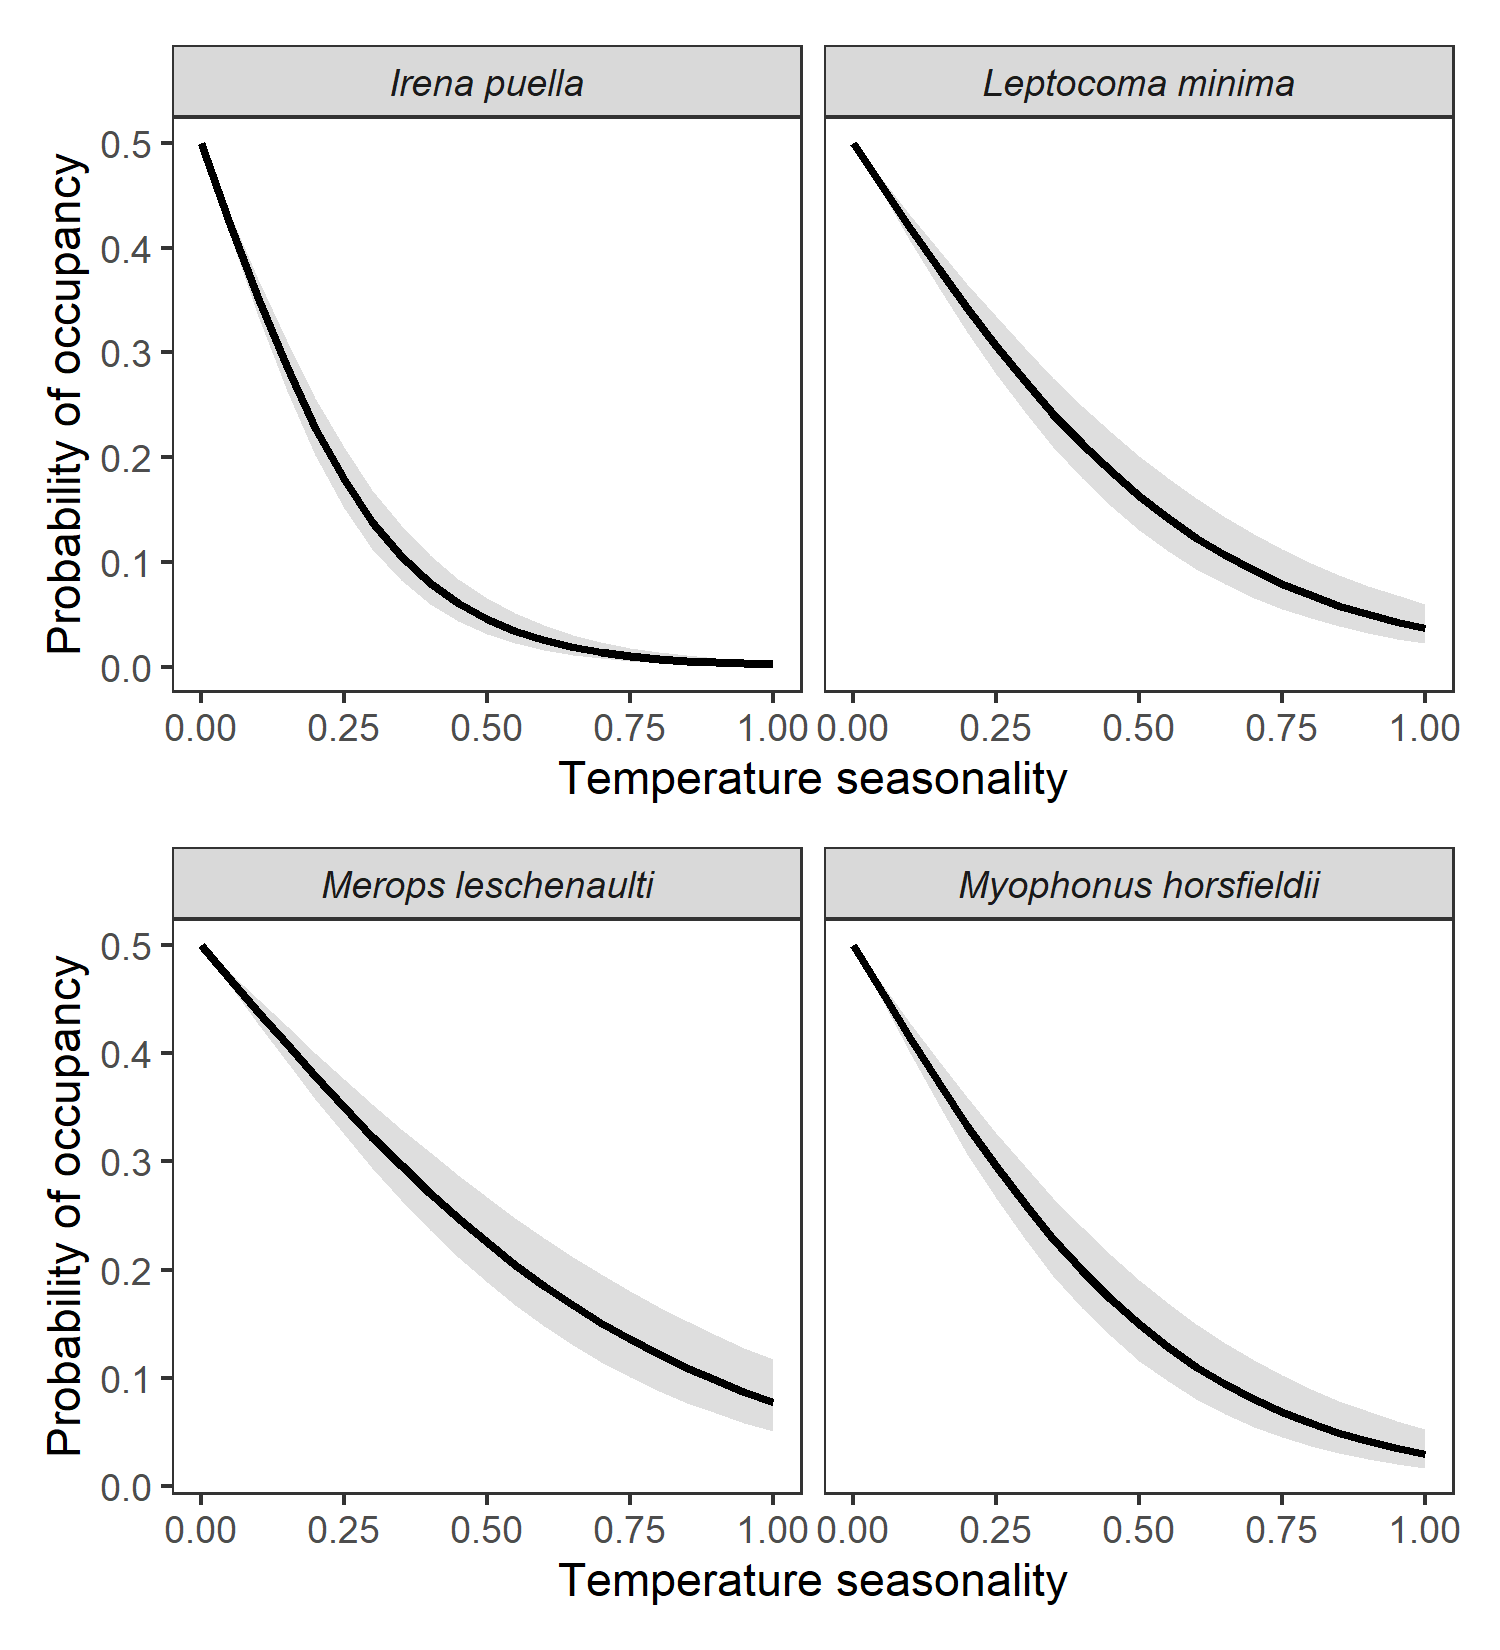
\includegraphics[width=0.95\textwidth]{figures/fig_05.png}
        \caption{
            \textbf{Thinning tracking data can aid computation but must be approached carefully}.\\
            Aggregating a filtered and smoothed movement track \textbf{(a)} preserves track structure while reducing data-volume, but \textbf{(b)} aggregating before filtering gross location errors and unrealistic movement leads to the persistence of large-scale errors (such as prolonged spikes).
            \textbf{(c)} Thinning before data cleaning can lead to significant misestimations of essential movement metrics such as speed at lower intervals.
            Boxplots show the median and interquartile ranges for speed estimates of tracks aggregated over intervals of 3, 10, 30, and 120 seconds.
            For comparison, the median and 95\textsuperscript{th} percentile of speed of the canonical track are shown as solid and dashed horizontal lines, respectively.
            % The unfiltered data would have to be thinned to \sfrac{1}{30}\textsuperscript{th} volume to correctly estimate median speed.
        }
        \label{fig:figure_thinning}
    \end{figure}

    \section*{System-Specific Pre-processing Tools}

    When researchers' pre-processing requirements exceed the functionalities of existing tools, they might have to conceptualise and implement their own methods.
    For instance, an important and common analysis with animal tracking data is to link space use with environmental covariates.
    This is difficult even with smoothed and thinned high-throughput data, as these may be too large for statistical packages, or have strong autocorrelation.
    Users aiming for such analyses can benefit from segmenting and clustering the data into spatio-temporally independent bouts of different behavioural modes \citep{patin2020a}.
    Treating these as the unit of observation also conveniently sidesteps pseudo-replication and reduces computational requirements.
    While numerous methods of segmenting and clustering data are in use, they may not be scalable to very large or gappy datasets \citep{patin2020a, langrock2012, michelot2016}.
    As an alternative, a first-principles approach that segments data based on the movement capacity (top speed, etc.) of tracked animals, could provide a fast, yet useful way to cluster data.
    Here, as a working example that may be suitable for some systems, we present a simple segmentation-clustering algorithm to make `residence patches', identified as bouts of relatively stationary behaviour \citep[][]{barraquand2008,bijleveld2016,oudman2018}.
    Details of the implementation may be found in the package code, and examples are provided in the Supplementary Material.

    \subsection*{Conceptualising a Simple Segmentation-Clustering Algorithm: The Residence-Patch Example}

    Before implementing the algorithm, users should identify positions where the animal is relatively stationary, for instance on its speed or first-passage time \citep{bracis2018,barraquand2008}.
    Our suggested algorithm begins by assessing whether consecutive stationary positions are spatio-temporally independent, and clusters them together into a residence patch if they are not.
    This clustering could be based on a simple proximity threshold --- points farther apart than some threshold distance are likely to represent two different residence patches.
    In cases where animals visit multiple sites in sequence \citep[such as traplining][]{thomson1997}, and which researchers might wish to consider as a single residence patch, a larger-scale distance threshold can help cluster nearby residence patches together, and this can also be applied to cluster together patches artificially separated due to missing data.
    Our algorithm separates two observations at a similar location, but at two very different time points, by comparing the intervening time-lag against a time-difference threshold, which can also apply to patches that would otherwise be clustered by the large-scale distance threshold.
    Users are encouraged to base these thresholds on the movement habits of their study species (see the \textit{Worked Out Example}).

    We have implemented a working example of the simple clustering concept presented here as the function \textit{atl\_res\_patch} (see Fig. 6.b; {\color{red} Listing} 6), which requires three parameters: (i) the distance threshold between positions (called \textit{buffer\_size}), (ii) the large-scale distance threshold between clusters of positions (called \textit{lim\_spat\_indep}), and (iii) the time-difference threshold between clusters (called \textit{lim\_time\_indep}).
    Clusters formed of fewer than a minimum number of positions can be excluded.
    Our algorithm performs well when movement modes are clearly separated, and is capable of correctly separating positions that are close together in space and time, but which comprise different behavioural sequences (see Fig. 6).
    While the algorithm may not cover all possible use-cases and study species, we provide it here as an example of a user-built exploratory method for animal tracking data.
    It is important to systematically test such custom-made algorithms, to ensure reproducibility and reliability \citep{wickham2015, marwick2018}.
    Simple examples of such tests for the residence patch method and other functions in \textit{atlastools} may be found in the \textit{tests/} directory in the associated Github repository.

    % \begin{lst{\color{red} Listing}}[float, language=R, style=customR, caption ={The \textit{atl\_res\_patch} function can be used to classify a track into residence patches. The arguments \textit{buffer\_radius} and \textit{lim\_spat\_indep} are specified in metres, while the \textit{lim\_time\_indep} is provided in minutes. In this example, specifying \textit{summary\_variables = c("speed")}, and \textit{summary\_functions = c("mean", "sd")} will provide the mean and standard deviation of instantaneous speed in each residence patch. The \textit{atl\_patch\_summary} function is used to access the classified patch in one of three ways, here using the \textit{summary} option which returns a table of patch-wise summary statistics.}]
    % patches <- atl_res_patch(
    %                 data = track_data,
    %                 buffer_radius = 10,
    %                 lim_spat_indep = 100,
    %                 lim_time_indep = 30,
    %                 min_fixes = 3,
    %                 summary_variables = c("speed"),
    %                 summary_functions = c("mean", "sd")
    %             )
    % \end{lst{\color{red} Listing}}

    % % patch_summary <- atl_patch_summary(
    % %                     patch_data = patches,
    % %                     which_data = "summary",
    % %                     buffer_radius = 10
    % %                 )

    % % first residence patch figure
    \begin{figure}[h!]
        \centering
        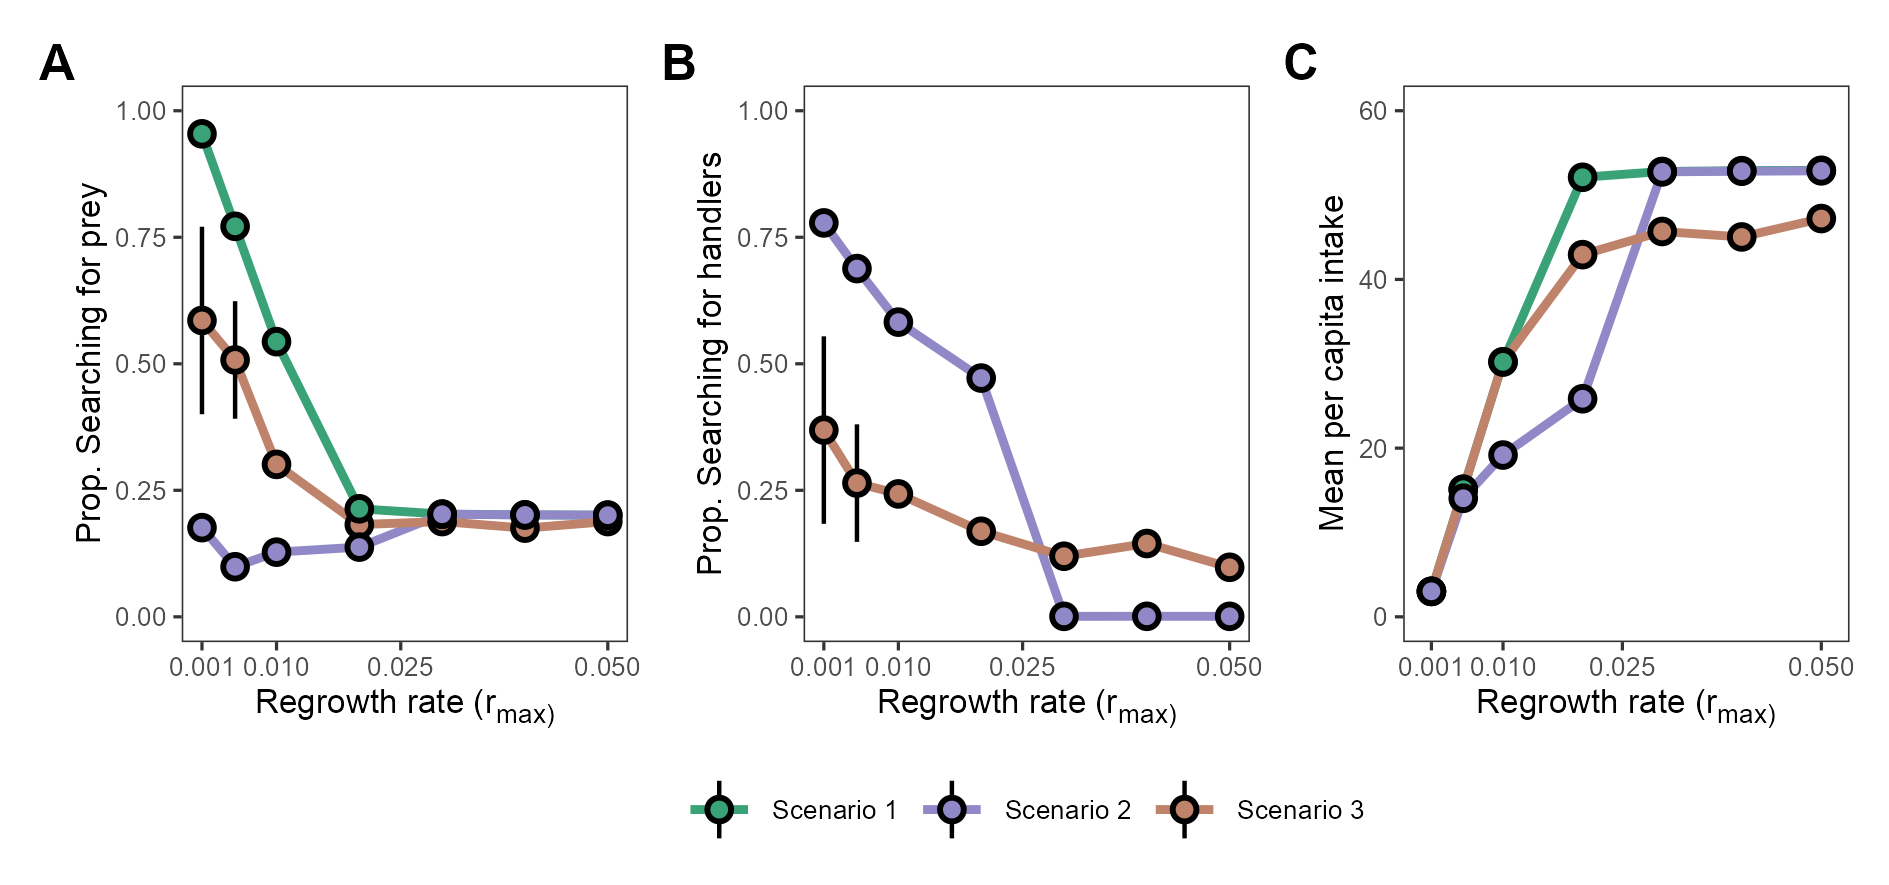
\includegraphics[width=0.75\textwidth]{figures/fig_06.png}
        \caption{
            \textbf{Movement tracks can be classified into residence patches, while leaving out the transit between them.}\\
            \textbf{(a)} A simulated animal movement track from \citealt{gupte2021a}, where an agent uses local cues to make movement decisions to maximise intake.
            The agent tends to stop (solid circles) on high-productivity areas of the landscape, as these are more likely to generate prey-items.
            Transit points between stationary phases are shown as crosses.
            \textbf{(b)} Our simple, first-principles based clustering algorithm classifies the track into five residence patches. 
            Some transit points are erroneously classified as being part of a residence patch (top, yellow), illustrating why is it important to remove such data before applying this method.
            Simultaneously, some points where the animal is not stationary for long are not picked up by the method.
            While the large purple patch (bottom) is composed almost entirely of consecutive positions, the subsequent patches are composed of multiple parts.
            This is because our method was designed to be robust to missing data from empirical tracks; the spatial and temporal limits of splitting and lumping can be controlled using the arguments passed to \textit{atl\_res\_patch}, and can be adjusted to fit the study system.
            Users are cautioned that there are no `correct' options, and the best guide is the behavioural biology of the tracked individual.
        }
        \label{fig:figure_residence_patch}
    \end{figure}

    \subsection*{A Real-World Test of User-Built Pre-Processing Tools}

    We applied the pre-processing pipeline using \textit{atlastools} functions described above to an ATLAS dataset to verify that the residence patch method could correctly identify known stopping points (see Fig. 7).
    We collected the data (n = 50,816) on foot and by boat, with a hand-held WATLAS tag (sampling interval = 1s) around the island of Griend (53.25$^{\circ}$N, 5.25$^{\circ}$E) in August 2020 \citep[WATLAS: Wadden Sea ATLAS system][Bijleveld et al. \textit{in prep.}]{beardsworth2021}.
    Since the data were intended to test the accuracy of the WATLAS system, we were able to log stops in the track as waypoints using a handheld GPS device, and manually annotate the WATLAS data with the timestamp of each waypoint (Garmin Dakota 10; see \citealt{beardsworth2021}).
    We estimated the real duration of each stop as the time difference between the first and last position recorded within 50m of each waypoint, within a 10 minute window before and after the waypoint timestamp (to avoid biased durations from revisits).
    Stops had a median duration of 10.28 minutes (range: 1.75 minutes -- 20 minutes; see Supplementary Material).
    We cleaned the data before constructing residence patches by (i) removing a single outlier ($>$ 15 km away), removing unrealistic movement ($\geq$ 15 m/s), smoothing the data ($K$ = 5), and (iv) thinning the data by subsampling over a 30 second interval.
    The cleaning steps retained 37,324 positions (74.45\%), while thinning reduced these to 1,803 positions (4.8\% positions of the smoothed track).
    Details and code are provided in the Supplementary Material (see \textit{Validating the Residence Patch Method with Calibration Data}).

    We began by visualising the data to check for location errors, and found a single outlier position approx. 15km away from the study area (Fig. 7.a).
    This outlier was removed by filtering data by the X coordinate bounds using the function \textit{atl\_filter\_bounds}; X coordinate bounds $\leq$ 645,000 in the UTM 31N coordinate reference system were removed (n = 1; remaining positions = 50,815).
    We then calculated the incoming and outgoing speed, as well as the turning angle at each position using the functions \textit{atl\_get\_speed} and \textit{atl\_turning\_angle} respectively, as a precursor to targeting large-scale location errors in the form of point outliers.
    We used the function \textit{atl\_filter\_covariates} to remove positions with incoming and outgoing speeds $\geq$ the speed threshold of 15 m/s (n = 13,491, 26.5\%; remaining positions = 37,324, 73.5\%; Fig. 7.b).
    This speed threshold was chosen as 5 m/s faster than the known boat speed, 10 m/s.
    Finally, we targeted small-scale location errors by applying a median smooth with a moving window size $K$ = 5 using the function \textit{atl\_median\_smooth} (Fig. 7.c).
    This step does not reduce the number of positions.

    We identified stationary positions as those where the median smoothed speed ($K$ = 5) was $<$ 2m/s, as people or a boat moving any faster are likely to be in transit.
    We clustered these positions into residence patches with a buffer radius of 5m, spatial independence limit of 50m, temporal independence limit of 5 minutes, and a minimum of 3 positions per patch.
    Inferred residence patches corresponded well to the locations of stops (see Fig. 7.c).
    However, the residence patch algorithm detected seven more stops (n = 28) than there were waypoints (n waypoints = 21).
    One of these was the field station on Griend where the tag was stored between trips (red triangle, Fig. 7.c), while another patch was formed of positions recorded while waiting for the boat; such unintended stops, not recorded as waypoints, likely accounted for the remaining five `extra' residence patches.
    Our analysis also did not detect two stops of 105 and 563 seconds (1.75 and 9.4 minutes) since they were data poor and were cleaned away during pre-processing (n positions = 6, 15), highlighting that the quality of the raw data (as in the rest of the track) is still a limiting factor on the inferences that are possible after pre-processing.
    To determine whether the residence patch method correctly identified the duration of detected stops in the calibration track, we first extracted the patch attributes using the function \textit{atl\_patch\_summary}.
    We then matched the patches to the waypoints by their median coordinates (rounded to 100 metres).
    We assigned the inferred duration of the stop as the duration of the spatially matched residence patch.
    We compared the inferred duration with the real duration using a linear model with the inferred duration as the only predictor of the real duration.
    % We excluded a single waypoint (WP080) since we had accidentally stopped there for $>$ 60 minutes.
    Inferred duration was a good predictor of the real duration of a stop (linear model estimate = 1.021, t-value = 12.965, $p <$ 0.0001, $R^2$ = 0.908; see Supplementary Material Fig.~\ref{fig1}.7).
    This translates to a 2\% underestimation of the stop duration at a tracking interval of 30 seconds.
    Finally, any classification algorithm will present users with a trade-off between over-sensitivity (erroneously finding stops where there were none), and under-sensitivity (missing stops where they are not local or long enough) --- users should balance between these based on the broader questions sought to be answered.

    % % calibration figure
    \begin{figure}[h!]
        \centering
        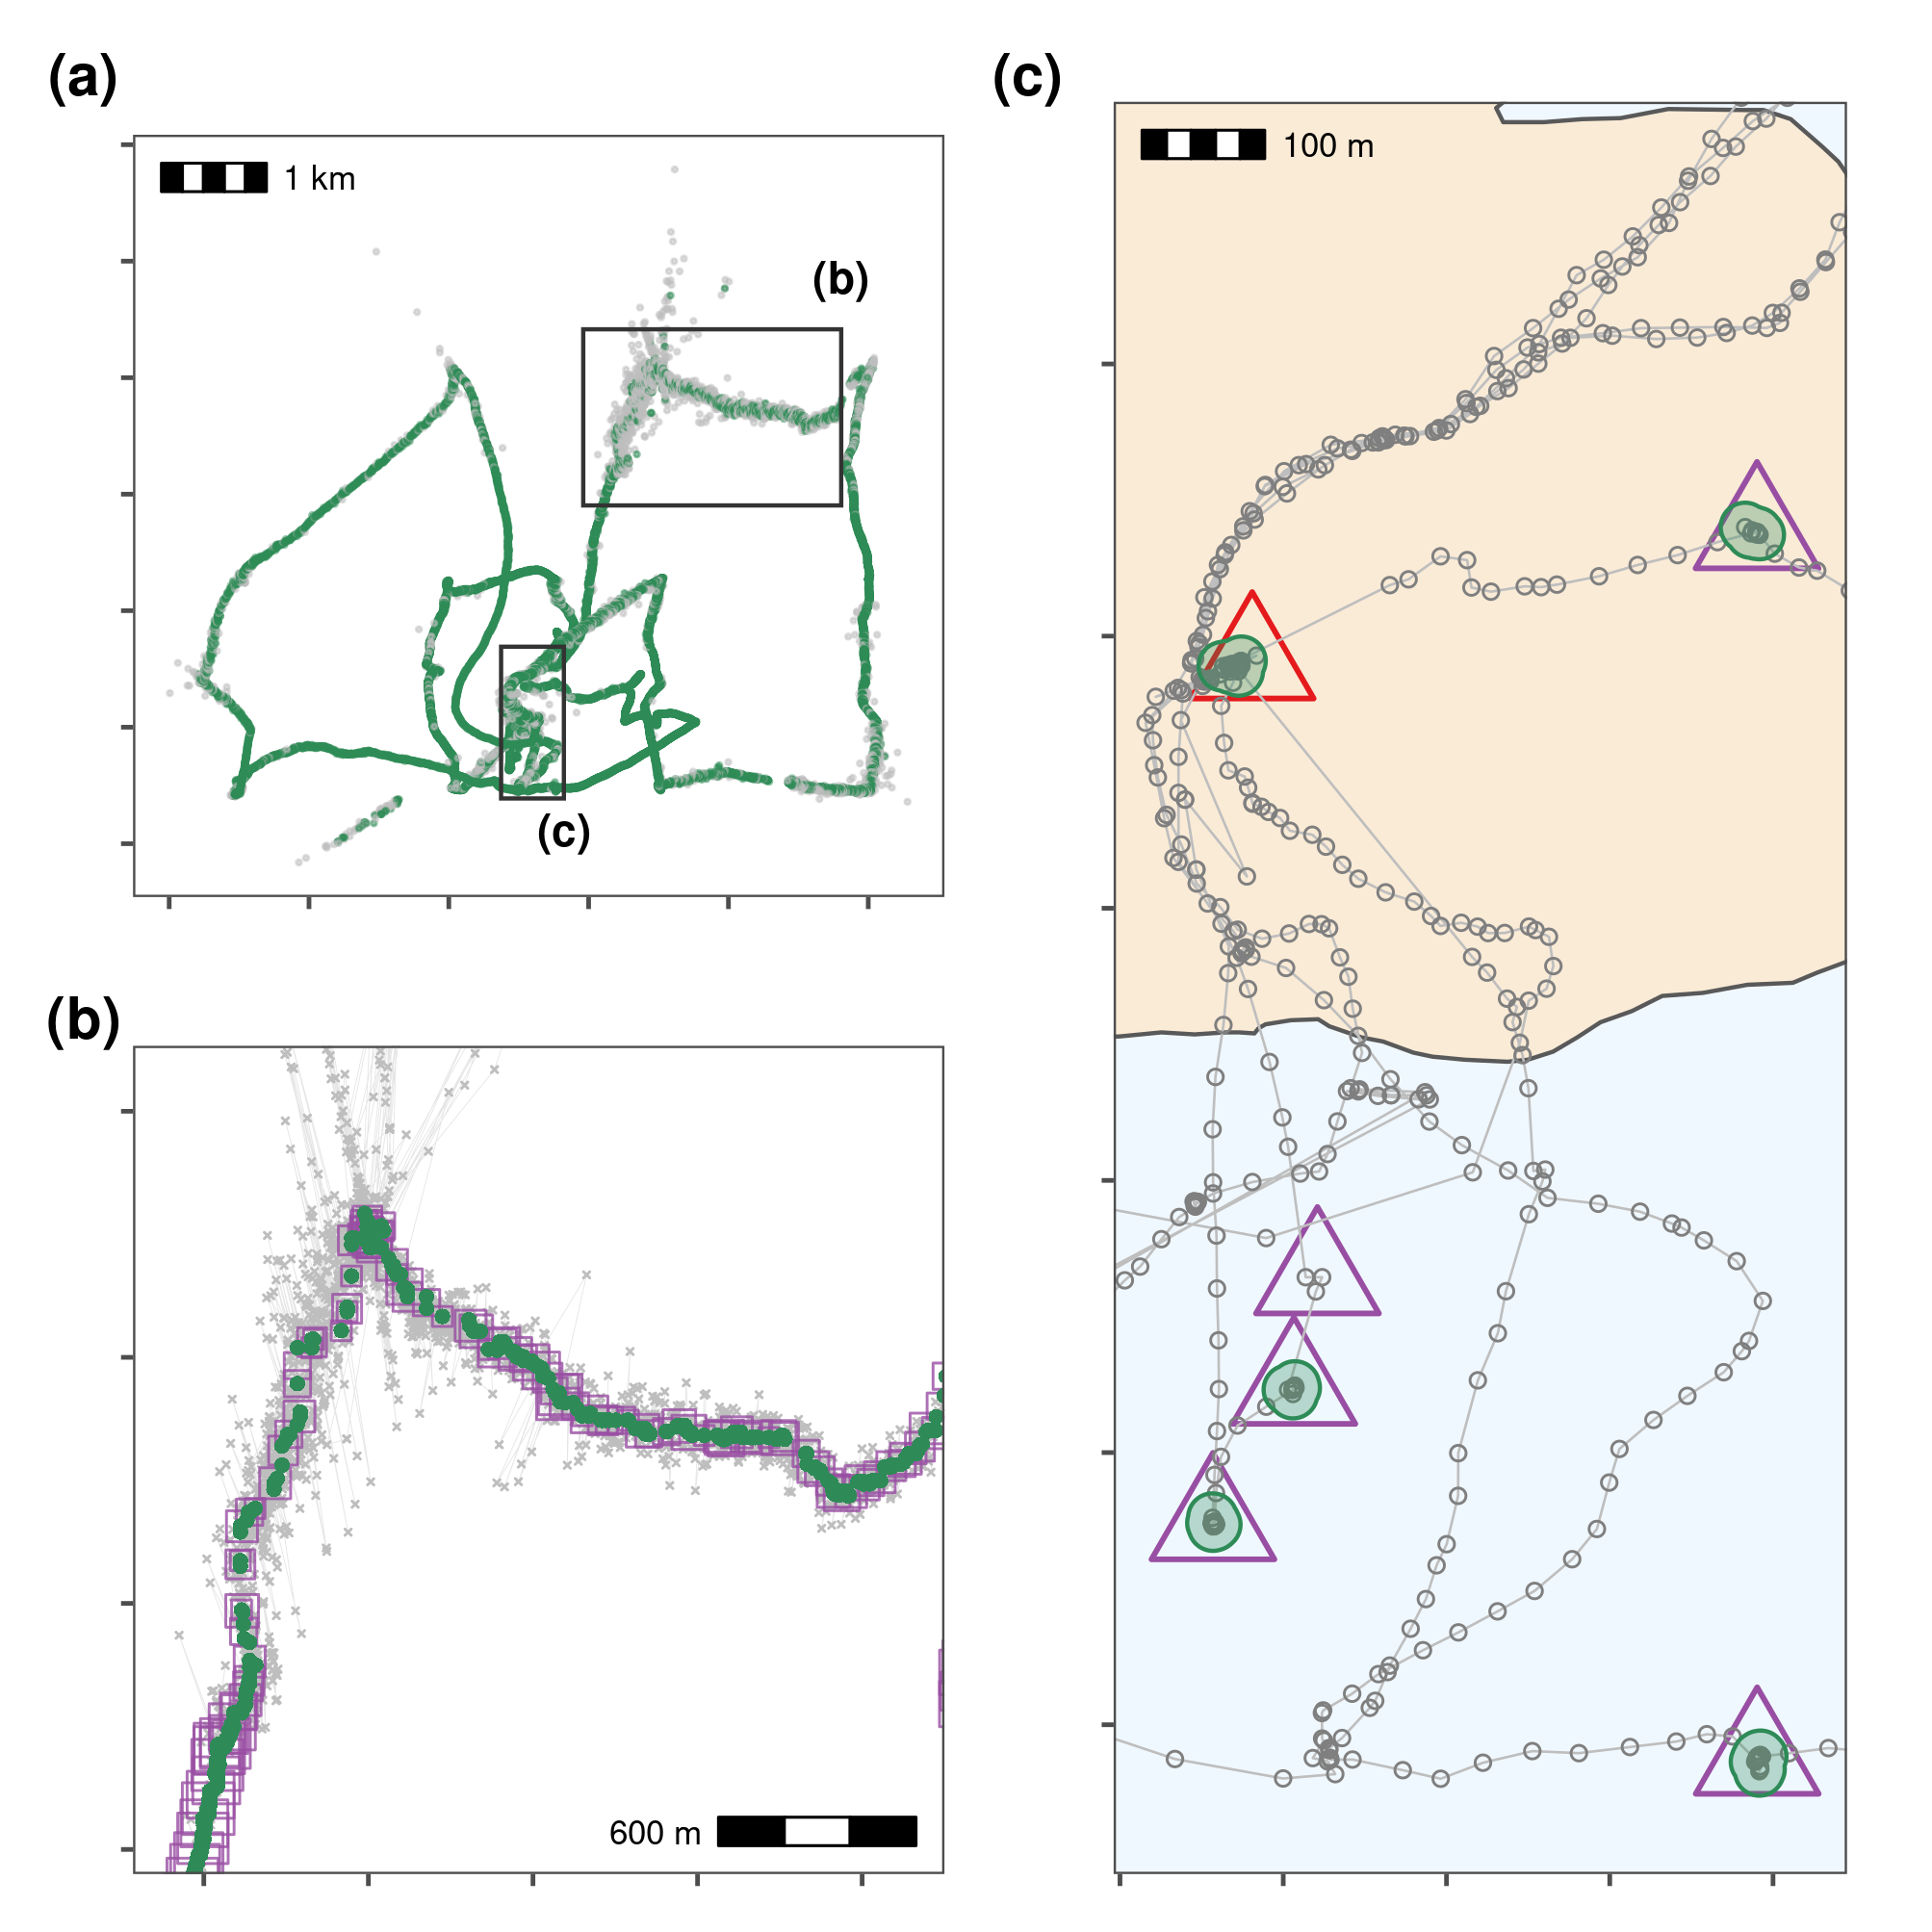
\includegraphics[width=0.75\textwidth]{figures/fig_07.png}
        \caption{
            \textbf{Pre-processing steps for WATLAS calibration data showing filtering on speed, median smoothing and thinning by aggregation, and making residence patches.}\\
            \textbf{(a)} Positions with incoming and outgoing speed $>$ 15 m/s are removed (grey crosses = removed, green points = retained).
            \textbf{(b)} Raw data (grey crosses), median smoothed positions (green circles; moving window $K$ = 5), and the smoothed track thinned by aggregation to a 30 second interval (purple squares).
            Square size corresponds to the number of positions used to calculate the averaged position during thinning.
            \textbf{(c)} Clustering thinned data into residence patches (green polygons) yields robust estimates of the location of known stops (purple triangles).
            The algorithm identified all areas with prolonged residence, including those which we had not intended to be recorded, such as stops at the field station (n = 12; red triangle).
            Our analysis could not find two stops of 105 and 563 seconds duration (6 and 15 fixes, respectively), since these were lost in the data thinning step; one of these is shown here (purple triangle without green polygon).
        }
        \label{fig:figure_calibration}
    \end{figure}

    \section*{A Worked-Out Example on Animal Tracking Data}

    We present a fully worked-out example of our pre-processing pipeline and residence patch method using movement data from three Egyptian fruit bats (\textit{Rousettus aegyptiacus}) tracked using the ATLAS system in the Hula Valley, Israel (33.1$^{\circ}$N, 35.6$^{\circ}$E) (\citealt{toledo2020, lourie2021}).
    Code and data can be found in the Supplementary Material and Zenodo repository (see \textit{Processing Egyptian Fruit Bat Tracks}). 
    Data selected for this example were collected over three nights (5\textsuperscript{th} -- 7\textsuperscript{th} May, 2018), with an average of 13,370 positions (SD = 2,173; range = 11,195 -- 15,542; interval = 8 seconds) per individual.
    Plotting the tracks revealed potential location errors (see Fig.~\ref{fig1}, see also Supplementary Material Fig.~\ref{fig2}.1), which we filtered out by removing observations with ATLAS SD $>$ 20 (see Supplementary Material Section 2.5), as well as removing observations calculated using fewer than four base stations, altogether trimming 22\% of the raw data (mean positions remaining = 10,447 per individual).
    % We converted the ATLAS time format (milliseconds since the UNIX Epoch) to the more common UNIX format (seconds since the Epoch) by taking the floored value of the time divided by 1000.
    Then, we removed unrealistic movement represented by positions with incoming and outgoing speeds $>$ 20 m/s that exceed the maximum flight speed recorded in this species (15 m/s; \citealt{tsoar2011}), leaving 10,337 positions per individual on average (98\% of previous step).
    We median smoothed the data with a moving window $K$ size = 5, and no observations were lost.

    We aimed to study bats' night-time foraging on fruit trees by quantifying the duration of bats' residence patches.
    We began the construction of residence patches by finding the residence time within 50 metres of each position; this is the maximal radius of a `cloud of points' around fruit trees \citep{bracis2018}.
    Foraging bats repeatedly traverse the same routes (\citealt{toledo2020, tsoar2011, lourie2021}) and this could artificially inflate the residence time of positions along these routes.
    To avoid confusing revisits with residence, we limited the summation of residence times at each position to the period until the first departure of 5 minutes or more.
    Thus, two nearby locations ($\leq$ 50m apart) each visited for one minute at a time, but separated by an interval of some hours would not be clustered together as a residence patch. 
    To focus on bats' night-time foraging behaviour, we also excluded positions during the day (5 AM -- 8 PM), and at or near the roost-cave (see Fig. 8a) to focus on night-time foraging behaviour; 22,910 of 31,012 positions remained (73.9\%).
    % Since bats departed and returned to their roost at different times each night, we also excluded locations with a residence time $>$ 200 minutes (approx. 3.3 hours), as this was more likely to represent daytime roosting than nighttime foraging; of 31,012 smoothed positions, 18,677 remained (60\%).
    % From these positions, we calculated that between leaving the roost to forage, and returning, bats had a mean residence time at each position of 95.64 minutes (SD = 119.23) --- this value is still likely to be biased by some positions at the roost.
    
    To determine the true duration of foraging, we opted for a first-principles approach and first selected only locations with a residence time $>$ 5 minutes, reasoning that a flying animal stopping for $>$ 5 minutes at a location should plausibly indicate resource use or another interesting localised behaviour.
    This step retained 5,736 positions per bat on average (17,208 total), or 72.4\% of the nighttime positions.
    We then constructed residence patches with a buffer distance of 25m, a spatial independence limit of 100m, a temporal independence limit of 30 minutes, and rejected patches with fewer than three positions.
    These values are meant as examples; users should determine the sensitivity of their results to parameter choices.
    Bats spent 56.95 minutes at foraging sites (SD = 62.20), and were stationary in particular fruit trees and roosting trees during 83.8\% of their foraging time (Fig. 8).
    Although all three bats roosted at the same cave during the day, and all their tracks are within the typical foraging area of bats roosting in this cave \citep{lourie2021}, they used distinct foraging sites across the area at night (Fig. 8.a). The lack of overlap among individuals in tree use, obtained with the residence patch algorithm, shows that although co-roosting bats share the same cave-specific foraging area \citep{lourie2021}, they often forage on different trees.
    Contrasting the actual movement path with the linear path between residence patches can help reveal details of how animal cognition affects space use \citep{toledo2020}.
    Bats tended to show prolonged residence near known food sources (fruit trees), but also where no fruit trees were recorded (Fig. 8.b, 8.c), in line with previous evidence for their use of non-fruiting trees to rest, to handle and digest food, and presumably for social interactions \citep{tsoar2011}.

    \begin{figure}[h!]
        \centering
        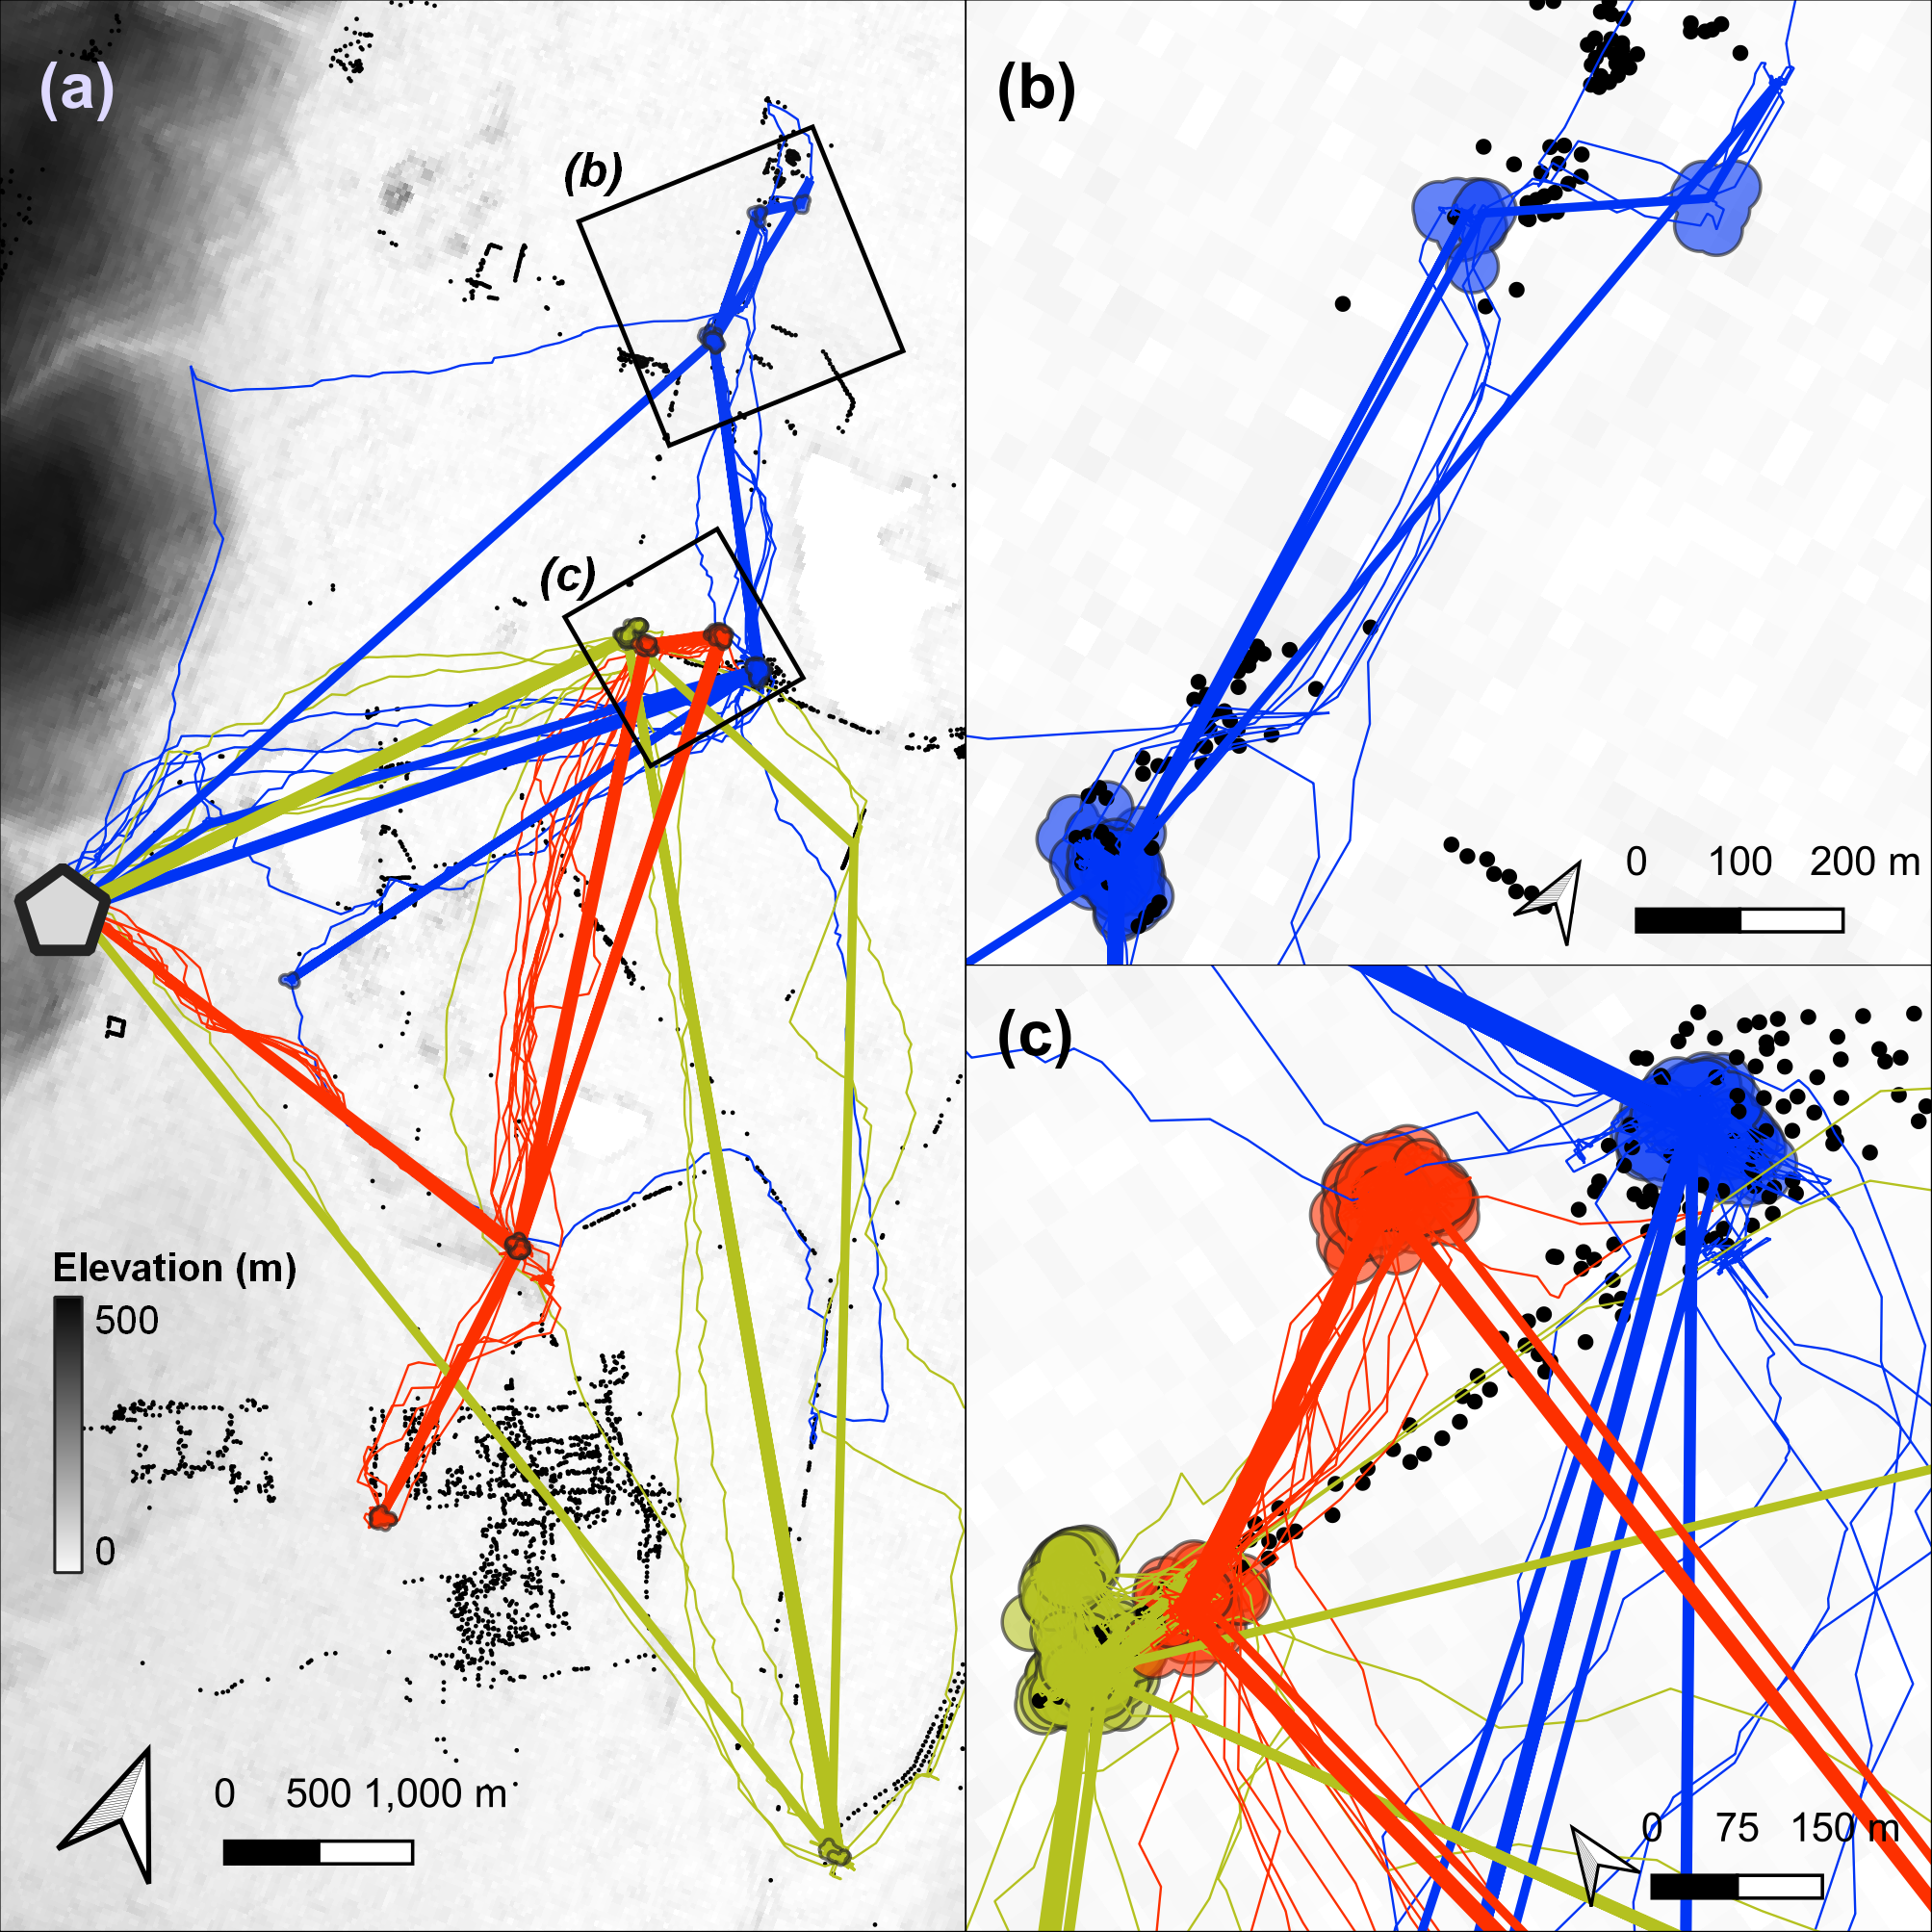
\includegraphics[width=0.75\textwidth]{figures/fig_08.png}
        \caption{
            \textbf{Synthesising animal tracks into residence patches can reveal movement in relation to landscape features, prior exploration, and other individuals.}
            \textbf{(a)} Linear approximations of the paths (coloured straight lines) between residence patches (circles) of three Egyptian fruit bats (\textit{Rousettus aegyptiacus}), tracked over three nights in the Hula Valley, Israel.
            Real bat tracks are are shown as thin lines below the linear approximations, and colours show bat identity. The grey hexagon represents the roost-cave at Gar Hershom.
            Black points represent known fruit trees.
            Background is shaded by elevation at 30 metre resolution.
            \textbf{(b)} Spatial representations of an individual bat's residence patches (green polygons) can be used to study site-fidelity by examining overlaps between patches, or to study resource selection by inspecting overlaps with known resources such as fruit trees (black circles).
            In addition, the linear approximation of movement between patches (straight green lines) can be contrasted with the estimated real path between patches (irregular green lines), for instance, to determine the efficiency of movement between residence patches.
            \textbf{(c)} Fine-scale tracks (thin coloured lines), large-scale movement (thick lines), residence patch polygons, and fruit tree locations show how high-throughput data can be used to study movement across scales.
            Patches and lines are coloured by bat identity.
        }
        \label{fig:figure_bats}
    \end{figure}

    \section*{Discussion and Perspective}

    Recent technical advances in wildlife tracking have already yielded exciting new insights from massive high-resolution movement datasets \citep{aspillaga2021, aspillaga2021a, baktoft2017, baktoft2019, harel2016, harel2018, oudman2018, papageorgiou2019, tsoar2011, strandburg-peshkin2015, toledo2020, beardsworth2021a, beardsworth2021b, corl2020, vilk2021, lourie2021}, and high-throughput animal tracking is expected to become increasingly more common in the near future.
    Tackling the very large datasets that high-throughput tracking generates requires a different approach from that used for traditionally smaller volumes of data.
    We foresee that movement ecologists will have to adopt ever more practices from fields accustomed to dealing with `big data', and that the field will become increasingly computational \citep{peng2011}.

    Researchers have long used some of these approaches \textit{ad hoc}, such as exploratory data analysis on small subsets before applying methods to the full data, using efficient tools, and basic batch-processing. 
    Yet formally prescribing these steps can help practitioners avoid pitfalls and implement techniques that make their analyses quicker and more reliable.
    Standardised principles, implemented a basic pipeline, for approaching data cleaning promote reproducibility across studies, making comparative inferences more robust.
    While massive datasets make reliance on standardised pipelines necessary, the output of such pipeline should periodically manually double-checked to ensure `realistic' output.
    The open-source \textit{R} package \textit{atlastools} serves as a starting point for methodological collaboration among movement ecologists, and as a simple working example on which researchers may wish to model their own tools.
    Efficient location error modelling approaches \citep{fleming2020, aspillaga2021} may eventually make data-cleaning optional.
    Yet cleaning tracking data even partially before modelling location error is faster than error-modelling on the full data, and the removal of large location errors may improve model fits.
    Thus we see our pipeline as complementary to these approaches \citep{fleming2014a, fleming2020}.

    Finally, we recognise that the diversity and complexity of animal movement and data collection techniques often requires system-specific, even bespoke, pre-processing solutions.
    Though the principles outlined here are readily generalised to numerous data sources (including terrestrial radio-based reverse-GPS: e.g. \citealt{toledo2020}, and marine acoustic reverse-GPS: e.g. \citealt{aspillaga2021}; high-resolution GPS such as \citealt{strandburg-peshkin2015}, and video-tracking: \citealt{rathore2020}), users' requirements will eventually exceed the particular tools we provide.
    % For instance, relational databases are the standard for storing very large datasets, and extending pre-processing pipelines to deal with various data sources is relatively simple, as we show in our Supplementary Material.
    We see the diversity of animal tracking datasets and studies as an incentive for more users to be involved in developing methods for their systems.
    We offer our approach to large tracking datasets, and our pipeline and package as a foundation for system-specific tools in the belief that simple, robust concepts are key to methods development that balances system-specificity and broad applicability.

    \printbibliography[title=Preprocessing,sorting=nyt,heading=subbibliography]
\end{refsection}